
\documentclass{article}
\usepackage{anyfontsize}
\usepackage[UTF8]{ctex} % 如果需要支持中文
\usepackage{fontspec} 
\setCJKmainfont{SourceHanSansCN-Light}[
    BoldFont=SourceHanSansCN-Medium
]

\usepackage[a4paper, left=0.1in, right=0.1in, top=0.05in, bottom=0.05in]{geometry} % 设置四边页边距为0.1英寸{geometry} % 设置页边距为0.5英寸



\usepackage{enumitem} % 用于自定义列表
\usepackage{amsmath}  % 数学公式支持
\usepackage[UTF8]{ctex} % 如果需要支持中文
\setlength{\parindent}{0pt} % 不缩进
\usepackage{etoolbox} % 用于列表操作
%调整类代码
\usepackage{comment}
\usepackage{tocloft} % 用于定制目录样式
\usepackage{hyperref} %不需要目录盒子注释这
\usepackage{ifthen}
\usepackage{titletoc}
\usepackage{graphicx}
\usepackage{float} 

\usepackage{tikz}
\usepackage{amsmath}
\usepackage{amssymb}
\usepackage{graphicx}
\usepackage{float}


\usepackage{pgfplots}
\pgfplotsset{compat=1.18}

% tikz额外库，用于更多绘图功能
\usetikzlibrary{arrows}
\usetikzlibrary{arrows.meta}
\usetikzlibrary{positioning}
\usetikzlibrary{calc}




%目录设定
%快捷键 CMD + / 注释
%  \renewcommand{\cftdot}{} % 隐藏目录中的页码
%  \cftpagenumbersoff{section}
%  \cftpagenumbersoff{subsection}
%  \makeatletter
%  \renewcommand{\@pnumwidth}{0em}  % 设置页码宽度为0
%  \renewcommand{\@tocrmarg}{0em}   % 设置右边距为0
%  \makeatother
 


\usepackage{environ}

\newif\ifshowcontent  % 定义一个条件判断变量
\showcontenttrue    % 设置为 false，隐藏所有 question 环境的内容

\newcounter{question} % 题目计数器
\setcounter{question}{0}
\NewEnviron{question}{%
    \ifshowcontent
        \par\stepcounter{question}\textbf{\thequestion.} \BODY\par % 如果显示内容，则输出
    \fi
}

\NewEnviron{choices}{%
    \ifshowcontent
        \begin{enumerate}[label=\Alph*., leftmargin=*]
            \BODY
        \end{enumerate}\par
    \fi
}

\NewEnviron{correctanswer}{%
    \ifshowcontent
        \textbf{答案:}\BODY\par
    \fi
}



\newenvironment{explanation}
{\textbf{解析:}\par}
{\par}



% 新增考察方面命令
\newcommand{\checklist}[1]{
    \textbf{考察:} #1 \par % 在题目下方显示考察方面
    \addcontentsline{toc}{subsection}{题号\thequestion 考察: #1} % 将考察内容添加到目录
    \vspace{2em} % 添加1em的垂直空间
}

\graphicspath{{images/}} %统一


\begin{document}
 %\fontsize{23}{31}\selectfont
 \tableofcontents % 添加目录
\newpage
%\pagestyle{empty}


\iftrue
\section{考点1:Modern Portfolio Theory}
\setcounter{question}{0}


\begin{question}
    Suppose Johnson and Johnson and Walgreen Company have the following expected returns and volatility, with a correlation coefficient of 22\%:

    \begin{center}
        \begin{tabular}{|l|c|c|}
            \hline
            \textbf{Stock} & \textbf{Expected Return} & \textbf{Volatility} \\
            \hline
            Johnson \& Johnson & 7\% & 16\% \\
            \hline
            Walgreens & 10\% & 20\% \\
            \hline
        \end{tabular}
    \end{center}

    If a portfolio consists of Johnson \& Johnson of \$8,000 and Walgreens of \$2,000, which of the following is the expected return and volatility of that portfolio?
\end{question}
    
    \begin{choices}
        \item Expected return: 7.6\%, Volatility: 14.23\%  
        \item Expected return: 8.0\%, Volatility: 15.00\%  
        \item Expected return: 7.6\%, Volatility: 13.50\%  
        \item Expected return: 8.5\%, Volatility: 16.00\%  
    \end{choices}

    \begin{correctanswer}
    A
    \end{correctanswer}
    
    \begin{explanation}
        \textbf{步骤1：计算投资组合的总投资}
        \begin{itemize}
            \item 总投资为：\$8,000 + \$2,000 = \$10,000
        \end{itemize}
    
        \textbf{步骤2：计算各资产的权重}
        \begin{itemize}
            \item 强生公司的权重：\(W_1 = \frac{8000}{10000} = 0.8\)
            \item 沃尔格林公司的权重：\(W_2 = \frac{2000}{10000} = 0.2\)
        \end{itemize}
    
        \textbf{步骤3：计算投资组合的预期收益}
        \begin{itemize}
            \item 投资组合的预期收益：
            \begin{align*}
            E[R_p] &= W_1 \times E[R_1] + W_2 \times E[R_2] \\
            &= 0.8 \times 7\% + 0.2 \times 10\% \\
            &= 7.6\%
            \end{align*}
        \end{itemize}
    
        \textbf{步骤4：计算投资组合的波动率}
        \begin{itemize}
            \item 投资组合的标准差计算公式：
            \begin{align*}
                SD(R_p) &= \sqrt{(W_1 \cdot SD[R_1])^2 + (W_2 \cdot SD[R_2])^2 + 2 \cdot W_1 \cdot{}} \\
                        &\phantom{= \sqrt{}} {W_2 \cdot SD[R_1] \cdot SD[R_2] \cdot \rho_{12}}
                \end{align*}
                \item 代入数值：
                \begin{align*}
                SD(R_p) &= \sqrt{(0.8 \cdot 0.16)^2 + (0.2 \cdot 0.20)^2 + {}} \\
                        &\phantom{= \sqrt{}} {2 \cdot (0.8)(0.2) \cdot 0.22(0.16)(0.20)}
            \end{align*}
            \item 计算得出：
            \[
            SD(R_p) \approx 14.23\%
            \]
        \end{itemize}
    
        因此，该投资组合的预期收益为7.6\%，波动率为14.23\%。
    \end{explanation}

\checklist{理解投资组合预期收益率和波动率的计算。(理解基础公式待入即可)}






\begin{question}
    A portfolio manager is considering adjusting the allocation of a two-asset portfolio. The current data for both assets is:

    \begin{center}
        \begin{tabular}{|l|c|c|}
            \hline
            \textbf{Asset Class} & \textbf{Expected Return} & \textbf{Volatility} \\
            \hline
            Fixed Income & 4.5\% & 15.0\% \\
            \hline
            Equities & 8.5\% & 22.0\% \\
            \hline
            \multicolumn{3}{|l|}{Correlation between assets = 0.35} \\
            \hline
        \end{tabular}
    \end{center}

    If the portfolio changes from an equal-weight allocation to 65\% equities and 35\% fixed income, what is the change in the portfolio's expected return?
\end{question}

\begin{choices}
    \item No change
    \item Increase of 0.65\%
    \item Increase of 1.30\%
    \item Increase of 1.95\%
\end{choices}

\begin{correctanswer}
    B
\end{correctanswer}

\begin{explanation}

    \textbf{步骤1：计算原始组合（等权重）的预期收益率。}
    \[
    R_{p1} = 50\% \times 4.5\% + 50\% \times 8.5\% = 6.5\%
    \]

    \textbf{步骤2：计算新组合（65\%股票，35\%债券）的预期收益率。}
    \[
    R_{p2} = 35\% \times 4.5\% + 65\% \times 8.5\% = 7.15\%
    \]

    \textbf{步骤3：计算预期收益率的变化。}
    \[
    \Delta R_p = R_{p2} - R_{p1} = 7.15\% - 6.5\% = 0.65\%
    \]

    \textbf{注意事项：}
    \begin{itemize}
        \item 组合预期收益率是各资产预期收益率的加权平均
        \item 波动率和相关系数不影响预期收益率的计算
        \item 权重之和必须等于100\%
    \end{itemize}

\end{explanation}

\checklist{理解组合预期收益率的计算.(不用考虑波动率和相关系数)}


\begin{question}
    A portfolio analyst at a mutual fund company is developing a pairs trading strategy using two highly liquid stocks. When analyzing the risk-return characteristics of different portfolio weights, 
    which of the following statements is MOST accurate?
\end{question}

\begin{choices}
    \item The diversification benefit reaches its maximum when the correlation coefficient approaches 0.5, assuming other parameters remain constant.
    
    \item The risk of any two-asset combination follows a linear relationship with the weights in mean-standard deviation space.
    
    \item The risk of a two-asset portfolio with no short selling constraints cannot be lower than that of the less risky asset.
    
    \item For a two-asset portfolio, the minimum variance weights can be determined through a closed-form solution using variances and correlation.
\end{choices}

\begin{correctanswer}
    D
\end{correctanswer}

\begin{explanation}
    \textbf{A选项错误。}
    \begin{itemize}
        \item 分散化收益在相关系数接近-1时达到最大，而不是0.5。相关系数越接近-1，分散化效果越好，这是因为负相关性能够更好地抵消个别资产的风险波动。
    \end{itemize}

    \textbf{B选项错误。}
    \begin{itemize}
        \item 两资产组合的风险与权重之间不是线性关系，而是呈现曲线形态。这是因为组合风险公式中包含了平方项和交叉项，导致风险曲线通常位于连接两个资产点的直线之下。
    \end{itemize}

    \textbf{C选项错误。}
    \begin{itemize}
        \item 即使在禁止卖空的情况下，两资产组合的风险也可能低于单个资产的最低风险。
        \item 举例：当资产A的$\sigma=10\%$，资产B的$\sigma=20\%$，如果相关系数$\rho<0.5$，组合风险可低于10\%，具体计算：当$\rho=0.1$时，将82.6\%配置于低风险资产可使组合波动率降至9.28\%。
    \end{itemize}

    \textbf{D选项正确。}
    \begin{itemize}
        \item 两资产组合的最小方差权重确实有明确的解析解。具体公式为：
        \[w_1 = \frac{\sigma_2^2 - \sigma_{12}}{\sigma_1^2 + \sigma_2^2 - 2\sigma_{12}}\]
        \item 这是两资产情况的独特优势，不需要使用复杂的数值优化方法。而多资产组合才需要使用数值优化方法。
    \end{itemize}
\end{explanation}

\checklist{两资产组合的基本性质。（理解最小方差组合权重的计算方法）}



\begin{question}
    A portfolio, invested in two assets with equal weights, has a volatility of 11.18\% when the covariance (and correlation) between the asset returns is zero. If the covariance increases from zero to 0.0160, while the weights and individual asset volatilities remain unchanged, what is the change to portfolio volatility?
\end{question}

\begin{choices}
    \item Increase by 3.14\%
    \item Increase by 6.29\%
    \item Increase by 12.65\%
    \item Increase by 15.81\%
\end{choices}

\begin{correctanswer}
    A
\end{correctanswer}

\begin{explanation}
    \textbf{步骤1：计算组合方差的变化}
    \begin{itemize}
        \item 使用组合方差公式：\(\sigma_p^2 = W_A^2\sigma_A^2 + W_B^2\sigma_B^2 + 2W_AW_B \text{Cov}_{AB}\)
        \item 由于初始协方差为零，方差变化为：\(\Delta \sigma_p^2 = 2W_AW_B \text{Cov}_{AB}\)
        \item 代入数值：\(\Delta \sigma_p^2 = 2 \times 0.5 \times 0.5 \times 0.016 = 0.008\)
    \end{itemize}

    \textbf{步骤2：计算组合的新方差}
    \begin{itemize}
        \item 初始方差为：\(11.18\%^2 = 0.0125\)，新方差为：\(\sigma_p^2 = 0.0125 + 0.008 = 0.0205\)
    \end{itemize}

    \textbf{步骤3：计算组合波动率的变化}
    \begin{itemize}
        \item 新波动率为：\(\sqrt{0.0205} \approx 14.32\%\)，波动率变化为：\(14.32\% - 11.18\% \approx 3.14\%\)
    \end{itemize}

    因此，组合波动率的变化为增加约3.14\%。
\end{explanation}

\checklist{理解组合波动率的变化。（组合波动率的变化与协方差的变化成正比）}












\begin{question}
    In modern portfolio theory, when plotting portfolios on a graph with risk (measured by standard deviation) on the horizontal axis and expected return on the vertical axis, what does the efficient frontier represent?
\end{question}

\begin{choices}
    \item All portfolios that achieve maximum returns regardless of their risk levels
    
    \item The set of portfolios that offer the highest expected return for each level of risk
    
    \item All portfolios with minimum risk levels regardless of their expected returns
    
    \item The collection of portfolios with extreme allocations that maximize either risk or return
\end{choices}

\begin{correctanswer}
    B
\end{correctanswer}

\begin{explanation}
    \textbf{A选项错误。}
    \begin{itemize}
        \item 仅关注最大化收益而忽视风险是不完整的。有效前沿强调的是在给定风险水平下的最优收益，而不是简单地追求最高收益。
    \end{itemize}

    \textbf{B选项正确。}
    \begin{itemize}
        \item 有效前沿代表了在每个风险水平下能够获得最高预期收益的投资组合集合。这些组合在风险-收益权衡中实现了最优化，没有其他组合能在相同风险下提供更高的收益。
        \item 相同风险水平下，收益越大越好；相同收益水平下，风险越小越好。
    \end{itemize}

    \textbf{C选项错误。}
    \begin{itemize}
        \item 有效前沿不仅仅关注最小风险组合。事实上，它包含了从最小方差组合到最高收益组合之间的一系列最优组合。
    \end{itemize}

    \textbf{D选项错误。}
    \begin{itemize}
        \item 极端配置并不一定是最优的。有效前沿上的组合是通过科学的优化过程得出的，而不是简单地选择极端值。
    \end{itemize}
\end{explanation}

\checklist{理解有效前沿的核心概念（相同风险水平下，收益越大越好；相同收益水平下，风险越小越好。）}




\begin{question}
    Consider the portfolio possibilities curve for stocks and bonds shown below. The expected return on stocks is 18\% (represented by point Z), and the expected return on bonds is 8\% (represented by point Y). Which point on the graph most likely represents a portfolio with a 90\% allocation in stocks and a 10\% allocation in bonds?
   
    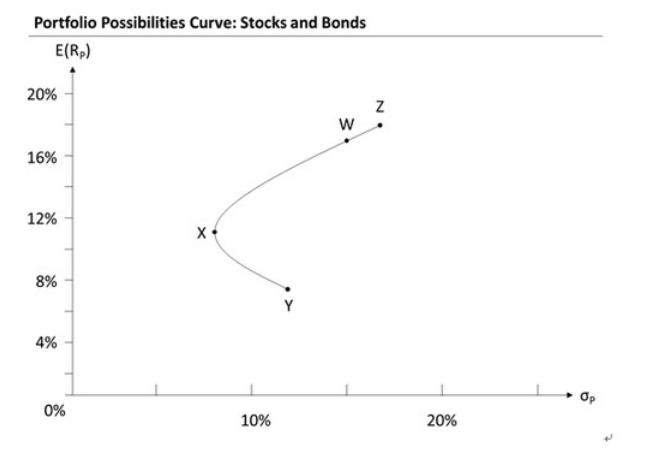
\includegraphics[width=0.5\textwidth]{images/有效边界第2题.jpg}
    
\end{question}

\begin{choices}
    \item W
    \item X
    \item Y
    \item Z
\end{choices}

\begin{correctanswer}
    A
\end{correctanswer}

\begin{explanation}
    \textbf{A选项正确。}
    \begin{itemize}
        \item W点最接近纯股票投资（Z点）的收益特征，同时显示出轻微的风险降低，这正是加入少量债券（10\%）的典型效果。其位置反映了保持高股票敞口同时获得适度分散化收益的投资组合特征。
    \end{itemize}

    \textbf{B选项错误。}
    \begin{itemize}
        \item X点位于曲线的中间位置，表明股票和债券的配置比例相对均衡，与90/10的极端配置不符。这种配置通常代表更保守的投资策略。
    \end{itemize}

    \textbf{C选项错误。}
    \begin{itemize}
        \item Y点代表100\%债券投资，收益率为8\%。这与要求的90\%股票配置完全相反，无法体现高股票配置的特征。
    \end{itemize}

    \textbf{D选项错误。}
    \begin{itemize}
        \item Z点代表100\%股票投资，收益率为18\%。虽然接近90/10的配置，但它代表的是纯股票投资，没有体现出任何债券配置的风险分散效果。
    \end{itemize}
\end{explanation}

\checklist{理解投资组合可能性曲线上不同点位的含义。（先考虑极端或者纯的情况）}




\begin{question}
    A risk manager is analyzing the characteristics of a portfolio created by combining two technology stocks with the following properties:

    \begin{center}
        \begin{tabular}{|l|c|}
            \hline
            \textbf{Characteristic} & \textbf{Value} \\
            \hline
            Stock A Standard Deviation & 16\% \\
            \hline
            Stock B Standard Deviation & 22\% \\
            \hline
            Correlation Coefficient & -1 \\
            \hline
        \end{tabular}
    \end{center}

    If no borrowing and no short selling is permitted, which of the following statements about the potential portfolios constructed from these two stocks is correct?
\end{question}

\begin{choices}
    \item The portfolio's risk level can potentially exceed the volatility of the more risky stock (22\%)
    
    \item Through optimal weighting, it is theoretically possible to construct a risk-free portfolio
    
    \item Every possible combination of these stocks will result in an optimal risk-return tradeoff
    
    \item The risk-return combinations of all possible portfolios will plot as a linear relationship
\end{choices}

\begin{correctanswer}
    B
\end{correctanswer}

\begin{explanation}
    \textbf{A选项错误。}
    \begin{itemize}
        \item 在不允许做空和借贷的限制下，投资组合的风险水平不可能超过风险最高的个股（22\%）。权重限制在0到1之间时，组合风险必然在两个股票的风险区间内。
    \end{itemize}

    \textbf{B选项正确。}
    \begin{itemize}
        \item 当两个资产完全负相关（相关系数为-1）时，存在一个最优权重组合，使得：
        \begin{itemize}
            \item 两个股票的波动方向完全相反
            \item 波动幅度可以通过权重精确调整
            \item 两股票的风险敞口能够完全对冲
        \end{itemize}
    \end{itemize}

    \textbf{C选项错误。}
    \begin{itemize}
        \item 并非所有的组合都是最优的。有效边界上的组合才是在特定风险水平下提供最高预期收益的最优组合。
    \end{itemize}

    \textbf{D选项错误。}
    \begin{itemize}
        \item 投资组合的基本特征：
            \begin{itemize}
                \item 收益率计算：$R_p = w_1R_1 + w_2R_2$（线性关系）
                \item 风险计算：$\sigma_p^2 = w_1^2\sigma_1^2 + w_2^2\sigma_2^2 + 2w_1w_2\sigma_1\sigma_2\rho_{12}$（非线性关系）
                \item 权重约束：$w_1 + w_2 = 1$
            \end{itemize}
        
        \item 在当前的限制条件下：
            \begin{itemize}
                \item 权重被限制在0到1之间
                \item 风险计算公式中的平方项导致非线性关系
                \item 可行组合只能形成一段连接两个原始资产点的弧线
            \end{itemize}
        
        \item 即使两资产完全负相关（$\rho_{12} = -1$），在有权重限制的情况下，风险-收益关系仍然不是线性的
    \end{itemize}
\end{explanation}

\checklist{理解完全负相关资产的投资组合特性。（风险-收益关系是弧线）}



\begin{question}
    During a portfolio theory lecture, Professor Zhang draws the portfolio possibilities curve (also known as the minimum-variance frontier) on the board. When discussing the mathematical properties of this curve in risk-return space, a student asks about its shape. Which of the following best describes the geometric characteristics of this curve?
\end{question}

\begin{choices}
    \item The entire curve exhibits a strictly convex shape, bending outward from the origin throughout its length
    
    \item The entire curve demonstrates a strictly concave shape, bending inward toward the origin at all points
    
    \item The curve is convex (bending outward) above the minimum variance portfolio and concave (bending inward) below it
    
    \item The curve is concave (bending inward) above the minimum variance portfolio and convex (bending outward) below it
\end{choices}

\begin{correctanswer}
    D
\end{correctanswer}

\begin{explanation}
   

    \textbf{A选项错误。}
    \begin{itemize}
        \item 如果整条曲线都是凸形的，就意味着风险和收益之间存在非理性的关系，违背了风险收益权衡的基本原则。实际上，理性投资者不会选择风险更高但收益相同或更低的组合。
    \end{itemize}

    \textbf{B选项错误。}
    \begin{itemize}
        \item 完全凹形的曲线暗示着可以通过降低风险来获得更高的收益，这违背了"高收益高风险"的基本投资原则，在现实市场中是不可能的。
    \end{itemize}

    \textbf{C选项错误。}
    \begin{itemize}
        \item 这个描述完全颠倒了曲线的实际形状。在最小方差点以上的有效边界部分应该是凹形的，以体现风险收益的边际效应递减规律。
    \end{itemize}

    \textbf{D选项正确。}
    \begin{itemize}
        \item 投资组合可能性曲线在最小方差点的上方呈凹形（向内弯曲），下方呈凸形（向外弯曲）。这种形状反映了现代投资组合理论的核心原理：在有效边界上（最小方差点以上的部分），投资者需要承担更多风险才能获得更高的预期收益，但这种收益增长是递减的。
    \end{itemize}

\end{explanation}

\checklist{理解投资组合可能性曲线形状的经济含义。（凹形是向内弯曲的，凸形是向外弯曲的）}



\begin{question}
    A portfolio manager is implementing Markowitz portfolio optimization for a new mutual fund. Which of the following inputs is least likely required for constructing the efficient frontier?
\end{question}

\begin{choices}
    \item Expected returns of individual securities in the investment universe
    \item Correlation matrix between all pairs of securities
    \item Average risk tolerance level of target investors
    \item Standard deviations of individual securities in the investment universe
\end{choices}

\begin{correctanswer}
    C
\end{correctanswer}

\begin{explanation}
    \textbf{A选项正确，不选。}
    \begin{itemize}
        \item 预期收益率是构建有效前沿的必要输入，用于计算组合预期收益，作为Markowitz模型的基本要素，不可或缺。
    \end{itemize}

    \textbf{B选项正确，不选。}
    \begin{itemize}
        \item 相关系数矩阵是必需的输入数据，用于计算组合风险，反映了资产间的分散化效应，是风险管理的关键。
    \end{itemize}

    \textbf{C选项错误。}
    \begin{itemize}
        \item 投资者的风险承受能力不是构建有效前沿所需的输入，风险偏好仅在有效前沿构建完成后，用于选择最优组合点。
    \end{itemize}

    \textbf{D选项正确，不选。}
    \begin{itemize}
        \item 标准差是必需的风险度量指标，用于计算组合风险，与相关系数共同构成有效前沿的基本统计输入。
    \end{itemize}
\end{explanation}

\checklist{理解Markowitz模型构建有效前沿。（预期收益率、相关系数、标准差是必需的，风险承受能力不是必需的）}





\begin{question}
    A portfolio manager is evaluating 15 potential stocks for a new fund launch. To construct the most efficient portfolio, the manager should:
\end{question}

\begin{choices}
    \item Allocate equal weights to all 15 stocks to maximize diversification.
    \item Select only stocks with below-average volatility to minimize portfolio risk.
    \item Identify the combination that provides the highest expected return for a given risk level.
    \item Exclude stocks that show strong negative correlations with the market.
\end{choices}

\begin{correctanswer}
    C
\end{correctanswer}

\begin{explanation}
    \textbf{A选项错误}
    \begin{itemize}
        \item 等权重配置虽然简单，但并不一定能实现组合的最优效率，因为它忽略了资产的个体特征，有效的投资组合应该根据资产间的相关性、个别风险和预期收益来确定最优权重，简单的等权重策略可能导致次优的风险收益组合。
    \end{itemize}

    \textbf{B选项错误}
    \begin{itemize}
        \item 仅考虑低波动性而忽略预期收益，违背了投资组合优化的基本原则，高波动性资产通过适当配置和相关性管理，也可能提高组合的整体效率，组合构建应同时考虑风险和收益两个维度。
    \end{itemize}

    \textbf{C选项正确}
    \begin{itemize}
        \item 符合有效前沿的定义：在给定风险水平下实现最高预期收益，或在给定收益目标下实现最低风险，体现了现代投资组合理论的核心原则：通过科学配置实现风险收益的最优权衡，考虑了所有相关因素：预期收益、风险水平、相关性结构和权重优化。
    \end{itemize}

    \textbf{D选项错误}
    \begin{itemize}
        \item 负相关性实际上是降低组合风险的有效工具，有助于实现分散化效应，排除负相关资产会显著减少分散化机会，可能导致组合效率降低，现代投资组合理论强调利用资产间的相关性结构来优化组合表现。
    \end{itemize}
\end{explanation}

\checklist{理解有效前沿的构建。（在给定风险水平下实现最高预期收益，或在给定收益目标下实现最低风险）}




\begin{question}
    A portfolio analyst at a pension fund is studying the characteristics of efficient portfolios constructed from two stocks X and Y. The following graph shows four possible portfolio opportunity curves in the mean-standard deviation space:

    \begin{center}
        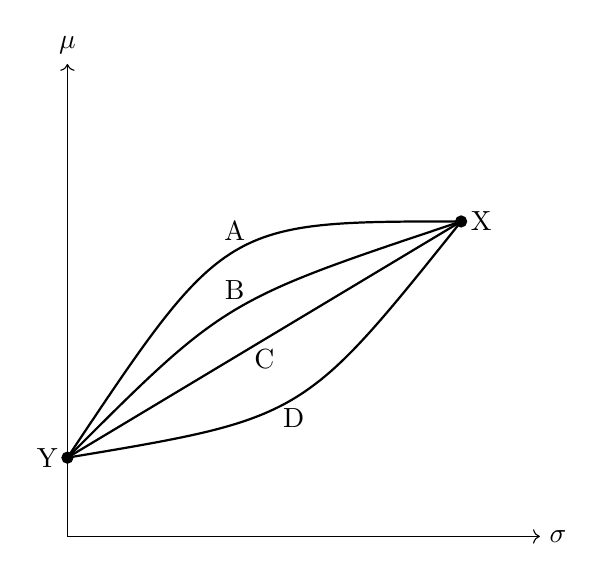
\begin{tikzpicture}
            % 坐标轴
            \draw[->] (0,0) -- (6,0) node[right] {$\sigma$};
            \draw[->] (0,0) -- (0,6) node[above] {$\mu$};
            
            % 点Y和X
            \filldraw (0,1) circle (2pt) node[left] {Y};
            \filldraw (5,4) circle (2pt) node[right] {X};
            
            % 四条曲线及其标签
            \draw[thick] (0,1) .. controls (2,4) .. (5,4) node[midway, above] {A};
            \draw[thick] (0,1) .. controls (2,3) .. (5,4) node[midway, above] {B};
            \draw[thick] (0,1) -- (5,4) node[midway, below] {C};
            \draw[thick] (0,1) .. controls (3,1.5) .. (5,4) node[midway, below] {D};
        \end{tikzpicture}
    \end{center}

    Which curve is least likely to represent the efficient frontier for portfolios combining stocks X and Y?
\end{question}

\begin{choices}
    \item Curve A, which is strongly convex throughout
    \item Curve B, which is moderately convex
    \item Curve C, which is linear
    \item Curve D, which is concave throughout
\end{choices}

\begin{correctanswer}
    D
\end{correctanswer}

\begin{explanation}
    有效前沿的形状反映了投资组合分散化的效果。在两资产组合的情况下，其特征有明确的理论依据。

    \textbf{步骤1：分析曲线特征}
    \begin{itemize}
        \item 曲线A：向外凸出，表现出典型的分散化效应
        \item 曲线B：温和的凸形，仍然体现分散化收益
        \item 曲线C：直线形态，表示完全正相关
        \item 曲线D：向内凹陷，违背了投资组合理论
    \end{itemize}

    \textbf{步骤2：理论验证}
    
    两资产组合的风险公式：
    \[
    \sigma_p = \sqrt{w_1^2\sigma_1^2 + w_2^2\sigma_2^2 + 2w_1w_2\sigma_1\sigma_2\rho_{12}}
    \]
    其中$\rho_{12}$为相关系数，$-1 \leq \rho_{12} \leq 1$

    当$\rho_{12} < 1$时，组合风险小于权重加权的单个资产风险，产生凸形曲线。

\end{explanation}

\checklist{有效前沿的几何特征。（理解分散化效应对投资组合风险的影响）}


\begin{question}
    A portfolio manager at a pension fund is exploring diversification strategies. She is considering adding a new asset class to an existing portfolio and is particularly interested in how correlation affects the efficient frontier. When the correlation between two assets in a portfolio is reduced, how does this impact the efficient frontier?
\end{question}

\begin{choices}
    \item The efficient frontier remains stable unless return expectations change, in which case it extends to the upper right with minimal risk impact.
    \item The efficient frontier shifts down and to the left, indicating increased portfolio risk due to negative correlation.
    \item The efficient frontier expands to the northwest, reflecting reduced portfolio risk while maintaining or potentially enhancing returns.
    \item The efficient frontier stays stable unless individual asset volatilities change, as it primarily depends on each asset's standard deviation.
\end{choices}

\begin{correctanswer}
    C
\end{correctanswer}

\begin{explanation}
    \textbf{A选项错误。}
    \begin{itemize}
        \item 有效前沿的形状和位置会随资产间相关性的变化而改变，相关性的变化直接影响组合风险，即使预期收益保持不变。
    \end{itemize}

    \textbf{B选项错误。}
    \begin{itemize}
        \item 相关性降低实际上会降低而不是增加组合风险，负相关性通常会增强分散化效应，有助于降低组合整体风险。
    \end{itemize}

    \textbf{C选项正确。}
    \begin{itemize}
        \item 当两资产相关性降低时，投资组合的风险会减小（向左移动）
        \item 基于公式：$\sigma_p = \sqrt{w_1^2\sigma_1^2 + w_2^2\sigma_2^2 + 2w_1w_2\sigma_1\sigma_2\rho_{12}}$
        \item 相关系数$\rho_{12}$降低会减小交叉项，从而降低总体风险。
    \end{itemize}

    \textbf{D选项错误。}
    \begin{itemize}
        \item 即使个别资产的波动率保持不变，相关性的变化也会影响有效前沿，组合风险不仅取决于个别资产的标准差，还受资产间相关性的显著影响。
    \end{itemize}
\end{explanation}

\checklist{相关性对投资组合分散化效应的影响。（相关性越低，分散化效应越强，组合风险越低）}





\begin{question}
    Two investors, Alice and Bob, have different risk preferences. Alice's indifference curve is steeper than Bob's, indicating their varying attitudes towards risk. Both investors prefer less risk to more and seek higher returns. Which of the following accurately describes the optimal portfolio position and risk aversion level for Alice compared to Bob?
    \begin{choices}
        \item Positioned lower on the efficient frontier; Lower risk aversion
        \item Positioned lower on the efficient frontier; Higher risk aversion
        \item Positioned higher on the efficient frontier; Higher risk aversion
        \item Positioned higher on the efficient frontier; Lower risk aversion
    \end{choices}
\end{question}

\begin{correctanswer}
    B
\end{correctanswer}

\begin{explanation}

    \textbf{B选项正确。}
    \begin{itemize}     
        \item 两位投资者都是风险厌恶型，这意味着他们都希望在相同的收益下承担更少的风险。风险厌恶程度可以通过无差异曲线的陡峭程度来衡量。
    
        \item Alice的无差异曲线比Bob的更陡峭，表示她的风险厌恶程度更高。
        \begin{align*}
            \text{陡峭度}(\text{Alice}) &> \text{陡峭度}(\text{Bob}) \\
            &\implies \text{风险厌恶}(\text{Alice}) > \text{风险厌恶}(\text{Bob})
            \end{align*}
    
        \item 在有效前沿上，投资者的无差异曲线与前沿的切点决定了他们的最优投资组合。Alice的无差异曲线更陡峭，意味着她的切点更靠近横轴的左侧。这表示她选择的投资组合中风险资产的比例较低：
        \[
        \text{切点位置}(\text{Alice}) < \text{切点位置}(\text{Bob})
        \]
    
        \item 因此，Alice的最优投资组合在有效前沿上更靠左，反映出她的高风险厌恶程度。她更倾向于选择低风险、低收益的组合，而Bob则可能选择高风险、高收益的组合。
    
        \item 综上所述，选项B正确：Alice的投资组合在有效前沿上位置较低，且她的风险厌恶程度较高。
    \end{itemize}
    
    \end{explanation}

\checklist{无差异曲线与有效前沿的切点组合。（无差异曲线越陡峭，风险厌恶程度越高）}




\begin{question}
    An investment manager is responsible for the asset allocation for its client. He collects information on all available combinations in the market as follows:

    \begin{center}
    \begin{tabular}{|c|c|c|}
    \hline
    Portfolio & Expected Return & Standard Deviation \\
    \hline
    1 & 4\% & 2\% \\
    2 & 6\% & 14\% \\
    3 & 4\% & 4\% \\
    4 & 10\% & 14\% \\
    \hline
    \end{tabular}
    \end{center}

    As a rational investor, which portfolios will be chosen?
    \begin{choices}
        \item 1 and 4.
        \item 1 and 3.
        \item 2 and 3.
        \item 3 and 4.
    \end{choices}
\end{question}

\begin{correctanswer}
    A
\end{correctanswer}

\begin{explanation}
   在现代投资组合理论中，马科维茨认为理性投资者的选择符合两个标准：
    \begin{enumerate}
        \item 在相同期望收益率情况下，选择标准差较小的组合。
        \item 在相同标准差情况下，选择期望收益率较大的组合。
    \end{enumerate}

    \textbf{步骤1：比较组合1和组合3}
    \begin{itemize}
        \item 两者期望收益率均为4\%。组合1的标准差为2\%，小于组合3的4\%。因此，组合1优于组合3。
    \end{itemize}
    
    \textbf{步骤2：比较组合2和组合4}
    \begin{itemize}
        \item 两者标准差均为14\%。组合4的期望收益率为10\%，大于组合2的6\%。因此，组合4优于组合2。
    \end{itemize}
    
    根据上述分析，组合1和组合4符合选择标准。因此，选项A正确。
\end{explanation}

\checklist{理性投资者选择资产和组合的标准。（在相同期望收益率情况下，选择标准差较小的组合；在相同标准差情况下，选择期望收益率较大的组合）}









\fi


%模版
\iftrue
\section{考点2:CAPM模型}
\setcounter{question}{0}


\begin{question}
    An investment advisor is explaining portfolio optimization to a client. According to the capital asset pricing model (CAPM), which of the following statements about the efficient frontier is MOST accurate?
\end{question}

\begin{choices}
    \item The capital market line represents the optimal combination of the risk-free asset and the zero-beta portfolio in mean-variance space.
    
    \item The capital market line's slope primarily reflects market liquidity conditions and trading volume patterns.
    
    \item The efficient frontier exhibits perfect linearity in mean-variance space when assets demonstrate strong positive correlations.
    
    \item The efficient frontier assumes no transaction costs, no taxes, a common investment horizon for all investors, and that the return distribution has no skewness.
\end{choices}

\begin{correctanswer}
    D
\end{correctanswer}

\begin{explanation}
    \textbf{A选项错误。}
    \begin{itemize}
        \item 资本市场线（CML）是连接无风险资产和市场组合的直线，而不是零贝塔组合。CML代表了投资者可以通过结合无风险资产和市场组合来实现的最佳风险-回报组合。
    \end{itemize}

    \textbf{B选项错误。}
    \begin{itemize}
        \item 资本市场线的斜率主要由市场风险溢价和市场组合的波动性决定，而不是由市场流动性和交易量决定。它反映了每单位风险所获得的额外回报。
    \end{itemize}

    \textbf{C选项错误。}
    \begin{itemize}
        \item 有效前沿在均值-方差空间中总是呈现曲线形态，即使资产间存在强正相关。这是因为投资组合风险的计算涉及平方项和交叉项，导致非线性关系。即使在完全正相关的情况下，风险与权重之间的关系也不是线性的。
    \end{itemize}

    \textbf{D选项正确。}
    \begin{itemize}
        \item 有效边界的假设确实包括没有交易成本和税收，所有投资者共享相同的投资期限，并且假设收益分布是对称的。这些假设构成了模型的基础框架，有助于简化分析和应用。
    \end{itemize}
\end{explanation}

\checklist{理解有效边界的基本假设。（没有交易成本和税收，投资者共享相同的投资期限，收益分布对称）}




\begin{question}
    On the capital market line (CML), how is a portfolio positioned to the right of the market portfolio constructed?
\end{question}

\begin{choices}
    \item Leveraging to invest more than 100\% in the market portfolio
    
    \item Achieving complete diversification of the portfolio
    
    \item Investing primarily in risk-free assets
    
    \item Combining risk-free assets with the market portfolio in equal proportions
\end{choices}

\begin{correctanswer}
    A
\end{correctanswer}

\begin{explanation}
    \textbf{A选项正确。}
    \begin{itemize}
        \item 要在CML上位于市场组合右侧，投资者必须通过借入资金（杠杆）投资超过100\%的市场组合。这种策略会增加投资组合的风险和潜在收益，使其在风险-收益图上向右上方移动。
    \end{itemize}

    \textbf{B选项错误。}
    \begin{itemize}
        \item 完全分散化是市场组合的固有特征，而不是获得更高风险收益的方法。事实上，市场组合已经是完全分散化的，无法通过进一步分散化来改变其风险-收益特征。
    \end{itemize}

    \textbf{C选项错误。}
    \begin{itemize}
        \item 增加无风险资产的比例会使投资组合在CML上向左移动（即向Rf点移动），而不是向右。这种策略会降低而不是增加投资组合的风险和预期收益。
    \end{itemize}

    \textbf{D选项错误。}
    \begin{itemize}
        \item 结合无风险资产和市场组合会创建位于市场组合左侧的投资组合。这种组合的风险和收益都低于市场组合，与题目要求相反。
    \end{itemize}
\end{explanation}

\checklist{理解CML上不同位置的投资组合构建方式。（市场组合右侧需要杠杆，左侧则是无风险资产和市场组合的组合）}



\begin{question}
    In Capital Market Theory, the optimal market portfolio represents the most efficient combination of all risky assets. According to the theory, how is this market portfolio specifically determined?
\end{question}

\begin{choices}
    \item By drawing a tangent line from any arbitrary point on the expected return axis to the efficient frontier
    
    \item By constructing a straight line from the origin to any portfolio located on the efficient frontier
    
    \item By identifying the point where a line from the risk-free rate is tangent to the efficient frontier
    
    \item By locating where the efficient frontier intersects with investors' highest attainable utility curve
\end{choices}

\begin{correctanswer}
    C
\end{correctanswer}

\begin{explanation}
    

    \textbf{A选项错误。}
    \begin{itemize}
        \item 切线必须从无风险利率点出发，而不是任意点，从其他点画出的切线无法确定最优的市场组合，这种方法忽视了无风险资产的重要性。
    \end{itemize}

    \textbf{B选项错误。}
    \begin{itemize}
        \item 从原点出发的直线没有经济意义，有效边界上的任意组合不一定是市场组合，这种方法忽略了风险溢价的概念。
    \end{itemize}

    \textbf{C选项正确。}
    \begin{itemize}
        \item 市场组合是从无风险利率点出发的切线与有效边界的切点，这个切点具有以下特征：
        \begin{itemize}
            \item 代表了风险资产的最优组合
            \item 形成了资本市场线(CML)
            \item 提供了最高的风险调整后收益
        \end{itemize}
    \end{itemize}

    \textbf{D选项错误。}
    \begin{itemize}
        \item 效用曲线是个人投资者的主观选择，市场组合的确定是客观的，不依赖于个人偏好，不同投资者的效用曲线会导致不同的交点。
    \end{itemize}
\end{explanation}

\checklist{理解市场组合的确定方法。（它是从无风险利率点到有效边界的切线的切点，这个位置代表了最优的风险资产组合）}




\begin{question}
    A portfolio manager is analyzing the effects of leverage on portfolio efficiency. Consider the following scenario:
    \begin{itemize}
        \item The market portfolio (M) contains only risky assets
        \item A risk-free asset exists in the market
        \item Initially: 100\% investment in M with Sharpe ratio $S_1$
        \item Subsequently: Borrows 40\% at risk-free rate to invest 140\% in M, resulting in Sharpe ratio $S_2$
    \end{itemize}

    Which of the following statements best describes the impact of this leveraged position on portfolio efficiency and Sharpe ratios?
\end{question}

\begin{choices}
    \item The portfolio becomes inefficient and $S_2$ is lower than $S_1$ due to increased leverage risk
    
    \item The portfolio remains efficient but $S_2$ decreases to reflect the higher risk exposure
    
    \item The portfolio becomes inefficient although $S_2$ equals $S_1$ due to borrowing constraints
    
    \item The portfolio remains efficient and $S_2$ equals $S_1$ despite the increased leverage
\end{choices}

\begin{correctanswer}
    D
\end{correctanswer}

\begin{explanation}
    \textbf{A选项错误。}
    \begin{itemize}
        \item 杠杆风险的增加并不会降低夏普比率。当投资者以无风险利率借入资金时，风险和超额收益会同比例增加：
        \begin{align*}
            S_2 &= \frac{E(R_p) - R_f}{\sigma_p} \\
            &= \frac{1.4[E(R_M) - R_f]}{1.4\sigma_M} \\
            &= \frac{E(R_M) - R_f}{\sigma_M} \\
            &= S_1
        \end{align*}
        \item 这个公式清楚地表明，杠杆倍数（1.4）在分子分母中相互抵消。
    \end{itemize}

    \textbf{B选项错误。}
    \begin{itemize}
        \item 虽然风险确实增加了，但夏普比率并不会降低。根据资本市场线方程：
        \[
        E(R_p) = R_f + \frac{E(R_M) - R_f}{\sigma_M} \sigma_p
        \]
        \item 风险($\sigma_p$)的增加会带来相应的预期收益增加，保持斜率（夏普比率）不变。
    \end{itemize}

    \textbf{C选项错误。}
    \begin{itemize}
        \item 借贷约束可能限制杠杆水平，但不会影响组合的效率性。只要是在CML上的组合，无论使用多少杠杆，都是有效的。这体现在CML的线性特征上：
        \[
        E(R_p) = R_f + 1.4[E(R_M) - R_f]
        \]
        \[
        \sigma_p = 1.4\sigma_M
        \]
    \end{itemize}

    \textbf{D选项正确。}
\begin{itemize}
    \item 这个选项准确描述了杠杆投资的两个关键特征：
        \begin{itemize}
            \item 效率性：杠杆组合位于CML上，因此保持有效
            \item 夏普比率：杠杆不改变风险调整后的收益比率
        \end{itemize}
    \item 经济含义：通过杠杆，投资者可以在CML上向上移动，风险和预期收益会同比例增加，单位风险所获得的超额收益（夏普比率）保持不变。
\end{itemize}
\end{explanation}



\checklist{理解CML方程的杠杆效应。（夏普比率不变性）}



\begin{question}
    A risk analyst at a fixed-income investment firm is currently evaluating various models to optimize portfolio performance. In this context, which of the following is a DIFFERENCE between the capital asset pricing model (CAPM) and the capital market line (CML)?
\end{question}

\begin{choices}
    \item CML includes risk-free assets, and CAPM also includes risk-free assets.
    \item CAPM applies only to efficient portfolios, while CML applies to individual securities and all types of portfolios.
    \item In CAPM, risk is measured as systematic risk (beta), while in CML, risk is measured as total risk (volatility).
    \item Both CAPM and CML assume that a portfolio is diversified and efficient, but CML in particular represents the risk-return trade-off of an effective portfolio.
\end{choices}


\begin{correctanswer}
    C
\end{correctanswer}

\begin{explanation}
    \textbf{A选项错误。}
    \begin{itemize}
        \item CML和CAPM都包含无风险资产，因此这一点不是它们之间的区别。
    \end{itemize}

    \textbf{B选项错误。}
    \begin{itemize}
        \item CAPM公式：\(E(R_i) = R_f + \beta_i (E(R_m) - R_f)\)，适用于个别证券和所有类型的投资组合。它关注的是系统性风险（\(\beta\)），不要求组合必须有效。
        \item CML公式：\(E(R_p) = R_f + \frac{E(R_m) - R_f}{\sigma_m} \sigma_p\)，仅适用于有效投资组合。CML描述了市场组合和无风险资产之间的最佳风险-回报权衡。
    \end{itemize}

    \textbf{C选项正确。}
    \begin{itemize}
        \item 在CAPM中，风险被衡量为系统性风险（\(\beta\)），这意味着CAPM关注的是市场风险对个别证券和投资组合的影响。
        \item CAPM公式：\(E(R_i) = R_f + \beta_i (E(R_m) - R_f)\)，强调的是证券的预期回报与其系统性风险之间的关系。
        \item 在CML中，风险被衡量为总风险（波动性），因为CML仅适用于有效投资组合，描述了市场组合和无风险资产之间的最佳风险-回报权衡。
        \item CML公式：\(E(R_p) = R_f + \frac{E(R_m) - R_f}{\sigma_m} \sigma_p\)，强调的是有效组合的总风险与预期回报之间的关系。
    \end{itemize}

    \textbf{D选项错误。}
    \begin{itemize}
        \item CAPM适用于所有类型的组合，包括非有效组合，并不要求组合必须是分散和有效的。
        \item CML假设组合是有效的，特别代表了有效投资组合的风险-回报权衡，连接无风险资产和市场组合。
        \item 因此，CML强调的是在有效组合中的风险-回报关系，而CAPM则适用于更广泛的组合类型。
    \end{itemize}
\end{explanation}

\checklist{CAPM和CML的区别。（CAPM适用于所有类型的组合，包括非有效组合，CML假设组合是有效的）}




\begin{question}
    A portfolio manager is explaining the relationship between the Markowitz efficient frontier and capital market line to junior analysts. When discussing how the efficient frontier changes after introducing risk-free assets, which of the following statements is correct?
    \end{question}
    
    \begin{choices}
        \item The capital allocation line (CAL) is obtained by combining any risky asset with the risk-free asset, with its slope representing the portfolio's Treynor ratio.
        \item Adding risk-free assets to a portfolio will result in lower returns compared to a pure risky asset portfolio, as risk-free returns drag down overall performance.
        \item The capital market line (CML) implies that investors should allocate their investments between risk-free assets and the market portfolio.
        \item The CML is a special case of CAL, with both combining risky and risk-free assets, but the risky component of CML has higher risk than that of CAL.
    \end{choices}
    
    \begin{correctanswer}
    C
    \end{correctanswer}
    
    \begin{explanation}
        \textbf{A选项错误。}
        \begin{itemize}
            \item CAL的斜率是夏普比率\(\frac{E(R_p)-R_f}{\sigma_p}\)而非特雷诺比率\(\frac{E(R_p)-R_f}{\beta_p}\)。CAL表示风险资产组合P与无风险资产组合时的可能收益和风险组合，其斜率衡量单位总风险的超额收益。
        \end{itemize}
        
        \textbf{B选项错误。}
        \begin{itemize}
            \item 引入无风险资产后，投资者可以通过杠杆操作在CAL上获得比原有效前沿更优的风险收益组合。例如，当投资者借入无风险利率的资金增加风险资产投资时，可获得\(E(R_p) = R_f + w[E(R_i)-R_f]\)的预期收益，其中w>1。
        \end{itemize}
        
        \textbf{C选项正确。}
        \begin{itemize}
            \item CML是最优CAL，表示\(E(R_p) = R_f + \frac{E(R_M)-R_f}{\sigma_M}\sigma_p\)，其中风险资产必须是市场组合M。根据两基金分离定理，所有投资者都应在CML上选择无风险资产和市场组合的某种组合，只是权重w因风险偏好不同而异。
        \end{itemize}
        
        \textbf{D选项错误。}
        \begin{itemize}
            \item CML的风险资产是市场组合M，其夏普比率\(\frac{E(R_M)-R_f}{\sigma_M}\)是所有可能CAL中最高的。因此CML不是风险更高，而是风险收益效率最优的CAL。
        \end{itemize}
    \end{explanation}
    
    \checklist{资本市场线与资本配置线的区别（两基金分离定理、夏普比率、特雷诺比率）}



    \begin{question}
        A wealth management firm is developing an automated portfolio advisory platform for their clients. In the algorithm design phase, the team is discussing how to incorporate the efficient frontier concept. When explaining to stakeholders how the platform will optimize client portfolios, which of the following statements about the efficient frontier would be most accurate?
    \end{question}

\begin{choices}
    \item Markowitz's theory assumes perfect capital markets where all traders can access available information costlessly, thus eliminating the need for return distribution assumptions.

    \item The Capital Market Line (CML) is a straight line connecting the risk-free asset with the zero-beta portfolio in the risk-return space.

    \item A portfolio composed of two risky assets will necessarily outperform a portfolio consisting of one risky asset and one risk-free asset.

    \item When investors move beyond the market portfolio point on the CML, they borrow at the risk-free rate to increase their investment position, aiming to achieve higher expected returns while taking on greater risk.
\end{choices}

\begin{correctanswer}
    D
\end{correctanswer}

\begin{explanation}
    \textbf{A选项错误。}
    \begin{itemize}
        \item 马科维茨理论确实假设市场是完美的，但仍需要对收益率分布做出假设，该理论假设收益率服从正态分布，这是计算投资组合风险和收益的基础，信息可及性和收益率分布是两个独立的假设，不能混为一谈。
    \end{itemize}
    
    \textbf{B选项错误。}
    \begin{itemize}
        \item CML是连接无风险资产和市场组合（而非零贝塔组合）的直线，市场组合的贝塔系数为1，代表系统性风险的基准，这条直线代表了在给定风险水平下最优的风险-收益组合。
    \end{itemize}
    
    \textbf{C选项错误。}
    \begin{itemize}
        \item 这个说法与两基金分离定理相矛盾，引入无风险资产后，投资者可以通过CML获得比纯风险资产组合更优的风险-收益组合，在相同风险水平下，包含无风险资产的组合可以获得更高的预期收益。
    \end{itemize}
    
    \textbf{D选项正确。}
    \begin{itemize}
        \item 这准确描述了CML上杠杆投资的机制，当投资者希望获得高于市场组合的收益时，可以通过无风险利率借入资金，增加风险敞口，获取更高的预期收益。这反映了风险与收益的基本权衡关系，投资者在追求更高收益时必须承担更高的风险。
    \end{itemize}

   
\end{explanation}

\checklist{CML的定义及其相关特性。（CML上杠杆投资的机制）}



\begin{question}
    A risk analyst at a fixed-income investment firm states that the efficient frontier refers to the set of portfolios that maximizes expected return at each level of volatility. According to the Capital Asset Pricing Model (CAPM), which of the following statements regarding the efficient frontier are correct?
\end{question}

\begin{choices}
    \item The slope of the Capital Market Line (CML) is always negative, with its steepness determined by the market risk premium and the volatility of the market portfolio.
    
    \item The CML suggests that the allocation between risk-free assets and the market portfolio depends on the investor's risk tolerance.
    
    \item Investors with the lowest risk aversion typically hold the risk asset portfolio with the minimum standard deviation on the efficient frontier.
    
    \item The efficient frontier allows for the possibility that the returns of different assets in a portfolio may not exhibit a consistent correlation.
\end{choices}

\begin{correctanswer}
   B
\end{correctanswer}

\begin{explanation}

    \textbf{A选项错误。}
    \begin{itemize}
        \item 资本市场线（CML）的斜率实际上是正的，而不是负的。CML的斜率表示风险资产的预期收益与其风险（波动性）之间的关系。
        \item CML的方程为：
        \[
        \bar{R}_e = R_F + \frac{\bar{R}_M - R_F}{\sigma_M} \cdot \sigma_e
        \]
        其中，\(\bar{R}_e\) 是有效投资组合的预期收益，\(R_F\) 是无风险利率，\(\bar{R}_M\) 是市场投资组合的预期收益，\(\sigma_M\) 是市场投资组合的波动性，\(\sigma_e\) 是有效投资组合的波动性。
        \item 从公式可以看出，CML的斜率为 \(\frac{\bar{R}_M - R_F}{\sigma_M}\)，这是一个正值，表明随着风险的增加，预期收益也会增加。
        \item 这一特性反映了风险与收益之间的基本关系，投资者在追求更高收益时必须承担更高的风险。因此，A选项的说法是错误的。
    \end{itemize}
    
    \textbf{B选项正确。}
    \begin{itemize}
        \item CML确实表明无风险资产与市场投资组合之间的配置取决于投资者的风险承受能力。
        \item 风险承受能力较高的投资者会倾向于持有更多的风险资产，以期获得更高的预期收益。
        \item 反之，风险承受能力较低的投资者则会选择更多的无风险资产，以降低投资组合的整体风险。
    \end{itemize}
    
    \textbf{C选项错误。}
    \begin{itemize}
        \item 风险厌恶程度最低的投资者通常会选择在有效边界上标准差最高的风险资产组合，以追求更高的预期收益，而非标准差最低的组合。
    \end{itemize}
    
    \textbf{D选项错误。}
    \begin{itemize}
        \item 有效边界的假设是投资组合中不同资产之间的回报率存在一定的相关性，通过多样化可以降低整体风险。
        \item 如果不同资产之间的回报率完全不相关，投资者将无法通过组合来降低风险，这与有效边界的理论相悖。
    \end{itemize}

\end{explanation}

\checklist{资本资产定价模型（CAPM）下有效边界的概念及其相关特性。（需要知道有效边界的前提假设）}


\begin{question}
    Suppose that the correlation of the return of a portfolio with the return of its benchmark is 0.6, the volatility of the return of the portfolio is 7\%, and the volatility of the return of the benchmark is 5\%. What is the beta of the portfolio?
\end{question}

\begin{choices}
    \item 0.84
    \item 0.72
    \item 0.60
    \item 1.20
\end{choices}

\begin{correctanswer}
    A
\end{correctanswer}

\begin{explanation}
    \textbf{以下公式用于计算贝塔（Beta）：}

  \[ \beta_P = \frac{Cov(R_P, R_M)}{\sigma^2_M} = \rho_{P,M}\frac{\sigma_P}{\sigma_M} \]

    \textbf{其中：}
    \begin{itemize}
        \item \(\beta_P\) 代表投资组合的贝塔值，
        \item \(Cov(R_P, R_M)\) 代表投资组合回报与市场回报之间的协方差，
        \item \(\sigma_M\) 代表市场基准的波动率，
        \item \(\rho_{P,M}\) 代表投资组合回报与市场回报之间的相关系数，
        \item \(\sigma_P\) 代表投资组合的波动率。
    \end{itemize}

    \textbf{步骤：将已知数值代入公式。}

    \[
    \beta = 0.6 \cdot \frac{0.07}{0.05}=0.6 \cdot 1.4=0.84
    \]
    因此，投资组合的贝塔值为 \(0.84\)。
\end{explanation}

\checklist{贝塔系数的计算方法。（中规中矩的题目，待入公式即可）}

\begin{question}
    In a financial seminar, a group of investors discusses their strategies based on the Capital Asset Pricing Model (CAPM). They are particularly interested in understanding how they can optimize their investment decisions over a single time period. According to CAPM, what do these investors seek to maximize in their investment strategies?
\end{question}

\begin{choices}
    \item The investors aim to grow their wealth significantly while also being cautious about extreme losses in their return distributions.
    \item The investors focus on increasing their wealth without worrying about the potential for extreme losses in their return distributions.
    \item The investors strive to maximize their expected utility while being mindful of the risks associated with extreme outcomes in their return distributions.
    \item The investors prioritize maximizing their expected utility without concern for the risks of extreme outcomes in their return distributions.
\end{choices}

\begin{correctanswer}
    D
\end{correctanswer}


\begin{explanation}
    \textbf{A选项错误。} 
    \begin{itemize}
        \item 尽管投资者可能希望显著增加财富，但CAPM假设投资者的决策基于期望效用，而不是单纯关注极端损失。因此，这个选项不符合CAPM的假设。
    \end{itemize}
    
    \textbf{B选项错误。} 
    \begin{itemize}
        \item 虽然投资者确实关注财富的增长，但CAPM强调的是期望效用的最大化，而不是单纯的财富增长。因此，这个选项不准确。
    \end{itemize}
    
    \textbf{C选项错误。} 
    \begin{itemize}
        \item 根据CAPM，投资者努力最大化他们的期望效用，但模型假设他们不考虑回报分布的极端结果。因此，这个选项不符合CAPM的理论。
    \end{itemize}
    
    \textbf{D选项正确。} 
    \begin{itemize}
        \item CAPM假设投资者在决策时只关注期望收益和方差，而忽略了极端结果的风险。因此，投资者优先考虑最大化他们的期望效用，而不关注极端结果的风险。（CAPM做了一些不切实际的假设。和其他的一样模型，当仅仅依赖CAPM的结果时，必须小心。）
    \end{itemize}
\end{explanation}

\checklist{CAPM模型的假设中的投资者在投资决策中追求的最大化目标。（不care尾部风险）}


\begin{question}
    A risk analyst, Robert, uses a two-factor model to estimate the volatility of a portfolio. The covariance matrix of the factors is specified as follows:

    \begin{table}[h]
        \centering
        \begin{tabular}{|c|c|c|}
            \hline
            & Equity Factor & Bond Factor \\
            \hline
            Equity Factor & 0.04000 & 0.01800 \\
            \hline
            Bond Factor & 0.01800 & 0.09000 \\
            \hline
        \end{tabular}
    \end{table}

    The portfolio has the following factor sensitivities (i.e., betas):
    \begin{itemize}
        \item 0.80 to the Global Equity Factor
        \item 0.40 to the Global Bond Factor
    \end{itemize}

    The volatility of the Portfolio is nearest to which value?
\end{question}

\begin{choices}
    \item 15.20\%
    \item 17.80\%
    \item 19.40\%
    \item 21.60\%
\end{choices}

\begin{correctanswer}
    C
\end{correctanswer}

\begin{explanation}
    \textbf{公式说明：}
    在多因子模型中，组合波动率的计算公式为：
    \[
    \sigma_P = \sqrt{VAR(P)}
    \]
    其中P为组合收益率：
    \[
    P = \sum_{i=1}^n \beta_i F_i
    \]
    则组合方差为：
    \[
    VAR(P) = \sum_{i=1}^n \sum_{j=1}^n \beta_i \beta_j COV(F_i, F_j)
    \]
    其中：
    \begin{itemize}
        \item $\beta_i, \beta_j$ 是组合对因子i和j的敏感度
        \item $F_i, F_j$ 是第i个和第j个因子的收益率
        \item $COV(F_i, F_j)$ 是因子i和j之间的协方差
        \item 当i=j时，$COV(F_i, F_i)$ 即为因子i的方差
    \end{itemize}

    \textbf{步骤1：确定已知数据}
    \begin{itemize}
        \item 股票因子方差：$VAR_E = 0.04000$
        \item 债券因子方差：$VAR_B = 0.09000$
        \item 因子间协方差：$COV_{EB} = 0.01800$
        \item 股票因子beta：$\beta_E = 0.80$
        \item 债券因子beta：$\beta_B = 0.40$
    \end{itemize}

    \textbf{步骤2：代入公式计算}
    \[
    \sigma_P = \sqrt{\beta_E^2 VAR_E + \beta_B^2 VAR_B + 2\beta_E \beta_B COV_{EB}}
    \]
    \[
    = \sqrt{(0.80)^2 \times 0.04 + (0.40)^2 \times 0.09 + 2 \times 0.80 \times 0.40 \times 0.018}
    \]
    \[
    = \sqrt{0.0256 + 0.0144 + 0.0115}
    \]
    \[
    = \sqrt{0.0515} = 0.194 = 19.4\%
    \]

    \textbf{步骤3：选择最接近的答案}
    \begin{itemize}
        \item 计算得到的19.4\%与选项C的19.40\%最为接近
    \end{itemize}
\end{explanation}

\checklist{多因子模型中组合波动率的计算公式及其应用(特别注意协方差项的处理)}




\begin{question}
    A portfolio manager at a large pension fund is reviewing their diversification strategy across different asset classes and correlations. Which of the following statements about diversification is NOT correct?
\end{question}

\begin{choices}
    \item By holding a sufficiently large and diversified portfolio, investors can reduce or eliminate company-specific risks through proper security selection.
    
    \item A well-diversified portfolio reduces the importance of events affecting individual stocks, leaving the portfolio primarily exposed to general market risk.
    
    \item Since diversification can be achieved at little or no cost, investors should not expect compensation for unnecessary exposure to firm-specific risks.
    
    \item Diversification should be considered a risk transfer strategy as it shifts investment risks across different assets, thereby reducing exposure to any single asset.
\end{choices}

\begin{correctanswer}
    D
\end{correctanswer}

\begin{explanation}
    

    \textbf{A选项正确。}
    \begin{itemize}
        \item 通过持有充分分散的投资组合，可以显著降低或消除非系统性风险，这种分散效应通过适当的证券选择来实现。
        \item 公司特有的风险包括会计欺诈、
        网络攻击，关键人员流失，或任何其他影响特定
        在不影响其他市场的情况下。
    \end{itemize}

    \textbf{B选项正确。}
    \begin{itemize}
        \item 分散投资的核心作用是降低非系统性风险（公司特定风险），如单个公司的经营风险或财务风险
        \item 但无法消除系统性风险（市场风险），这种风险会影响整个市场的所有证券。
    \end{itemize}

    \textbf{C选项正确。}
    \begin{itemize}
        \item 根据现代投资组合理论：
        \begin{itemize}
            \item 由于分散投资成本低廉且容易实现，市场不会对可分散的非系统性风险提供风险溢价
            \item 理性投资者应该通过分散投资来消除这种可分散风险，而不是期望从中获得补偿
        \end{itemize}
        \item 风险补偿的来源：  
        \begin{itemize}
            \item 投资者获得的风险补偿（风险溢价）仅来自于无法通过分散投资消除的系统性风险
            \item 这符合CAPM的核心思想：只有系统性风险（用$\beta$衡量）才会被市场定价和补偿
        \end{itemize}
    \end{itemize}

    \textbf{D选项错误。}
    \begin{itemize}
        \item 分散投资是风险降低(reduction)而非风险转移(transfer)的方法
        \item 风险转移指将风险转给其他方（如通过保险或衍生品），而分散投资是通过组合来降低风险
    \end{itemize}

\end{explanation}

\checklist{理解多元化在风险管理中的作用。（多元化是降低风险的技术）}


\begin{question}
    Assume two portfolios, (A) and (B), are each well-diversified and the economy has only one factor. The expected return of portfolio (A) is 8.0\% and its beta is 1.30. The expected return of portfolio (B) is 6.0\% and its beta is 0.90. What is the implied risk-free rate?
\end{question}

\begin{choices}
    \item 1.50\%
    \item 2.25\%
    \item 3.00\%
    \item 5.75\%
\end{choices}

\begin{correctanswer}
    A
\end{correctanswer}

\begin{explanation}
    根据单因素模型（CAPM），我们可以建立两个方程：

    \textbf{步骤1：列出CAPM方程}
    \begin{itemize}
        \item Portfolio A: 8.0\% = R(f) + (1.30 × RP)
        \item Portfolio B: 6.0\% = R(f) + (0.90 × RP)
    \end{itemize}

    \textbf{步骤2：求解两个未知数}
    \begin{itemize}
        \item 两式相减消除R(f)：
            2.0\% = 0.40 × RP
        \item 求得风险溢价RP：
            RP = 2.0\% ÷ 0.40 = 5.0\%
        \item 代入任一方程求R(f)：
            8.0\% = R(f) + (1.30 × 5.0\%)
            8.0\% = R(f) + 6.5\%
            R(f) = 1.50\%
    \end{itemize}

    因此，隐含的无风险利率为1.50\%。

\end{explanation}

\checklist{掌握如何通过CAPM方程组求解隐含的无风险利率和市场风险溢价。（二元一次方程组）}



\begin{question}
    A newly launched hedge fund, the Global Alpha Fund, reports an expected annual return of 9.2\% with a volatility of 9.5\%. The fund uses the MSCI World Index as its benchmark, which has an expected annual return of 8.0\% and volatility of 11.2\%. If the risk-free rate is 2.5\% per year, what is the beta of the Global Alpha Fund according to the Capital Asset Pricing Model (CAPM)?
\end{question}

\begin{choices}
    \item 0.92
    \item 1.08
    \item 1.15
    \item 1.24
\end{choices}

\begin{correctanswer}
    C
\end{correctanswer}

\begin{explanation}
    当我们无法获得基金与基准指数之间的相关性或协方差时，可以使用CAPM模型反推beta值。

    \textbf{CAPM公式：}
    \[
    E(R_i) = R_f + \beta_i[E(R_M) - R_f]
    \]

    其中：\\
    - $E(R_i)$ = 基金预期收益率 = 9.2\%\\
    - $R_f$ = 无风险利率 = 2.5\%\\
    - $E(R_M)$ = 市场预期收益率 = 8.0\%

    \textbf{步骤1：代入已知数值}
    \[
    9.2\% = 2.5\% + \beta_i(8.0\% - 2.5\%)
    \]

    \textbf{步骤2：求解beta}
    \[
    9.2\% - 2.5\% = \beta_i(5.5\%)
    \]
    \[
    \beta_i = \frac{6.7\%}{5.5\%} = 1.15
    \]

    \textbf{验证合理性：}\\
    - 基金收益率(9.2\%)高于市场收益率(8.0\%)\\
    - 基金波动率(9.5\%)低于市场波动率(11.2\%)\\
    - beta为1.15表明基金对市场变动较为敏感，这与对冲基金的积极投资策略相符

\end{explanation}

\checklist{掌握CAPM公式反推beta值。（理解beta值与基金风险收益特征的关系）}


\begin{question}
    In the Capital Asset Pricing Model (CAPM), beta measures a stock's systematic risk relative to the market. When analyzing a stock's beta coefficient, which of the following statements is TRUE? A beta greater than one:
\end{question}

\begin{choices}
    \item Indicates the stock is risky and should be avoided, while a beta less than one indicates the stock is risk-free and safe for investment
    
    \item Indicates the stock is more sensitive to market movements than average, while a beta less than one indicates less sensitivity to market movements
    
    \item Suggests the stock is trading above its intrinsic value, while a beta less than one suggests the stock is trading below its intrinsic value
    
    \item Implies the stock will outperform in all market conditions, while a beta less than one implies consistent underperformance
\end{choices}

\begin{correctanswer}
    B
\end{correctanswer}

\begin{explanation}
    教材上的相关说法是：市场贝塔等于
    1. 任何贝塔系数为1的证券都与市场呈一对一的关系。
    因此，任何贝塔系数大于1的证券都有较大的波动
    市场风险较大)，被称为周期性（如奢侈品股）。任何安全
    贝塔系数低于1的股票被称为防御性股票（例如公用事业股）。周期性股票
    在经济扩张时期表现更好，而防御型股票在衰退时期表现更好。

    \textbf{A选项错误。}
    \begin{itemize}
        \item beta只衡量系统性风险，而不是总风险，beta小于1的股票并非无风险，它们仍然面临市场风险，只是程度较小，没有股票是完全无风险的。
    \end{itemize}

    \textbf{B选项正确。}
    \begin{itemize}
        \item beta系数衡量个股对市场波动的敏感度：
            \begin{itemize} 
                \item beta > 1：股票的波动幅度大于市场，即对市场变动更敏感
                \item beta < 1：股票的波动幅度小于市场，即对市场变动不太敏感
                \item beta = 1：股票的波动幅度与市场一致
            \end{itemize}
    \end{itemize}

    \textbf{C选项错误。}
    \begin{itemize}
        \item beta是风险指标，不能用来判断股票的估值水平，股票的高估或低估应该通过基本面分析来判断，beta与股票的内在价值没有直接关系。
    \end{itemize}

    \textbf{D选项错误。}
    \begin{itemize}
        \item 高beta股票在牛市可能表现更好，但在熊市可能跌得更深，低beta股票在熊市可能有更好的防御性，但在牛市可能涨幅较小，beta不能预测股票在所有市场条件下的表现。
    \end{itemize}
\end{explanation}

\checklist{beta系数的含义（beta系数的本质是衡量个股相对于市场的系统性风险）}


\begin{question}
    An analyst at CAPM Research Inc. is projecting a return of 21\% on Portfolio A. The market risk premium is 11\%, the volatility of the market portfolio is 14\%, and the risk-free rate is 4.5\%. Portfolio A has a beta of 1.5. According to the Capital Asset Pricing Model (CAPM), which of the following statements is true?
\end{question}

\begin{choices}
    \item The expected return of Portfolio A is greater than the expected return of the market portfolio
    
    \item The expected return of Portfolio A is less than the expected return of the market portfolio
    
    \item The return of Portfolio A has lower volatility than the market portfolio
    
    \item The expected return of Portfolio A is equal to the expected return of the market portfolio
\end{choices}

\begin{correctanswer}
    A
\end{correctanswer}

\begin{explanation}
    \textbf{A选项正确。}
    \begin{itemize}
        \item 根据CAPM模型：$E(R_A) = R_f + \beta[E(R_M) - R_f] = 4.5\% + 1.5 \times 11\% = 21\%$
        \item 市场组合预期收益率：$E(R_M) = 11\% + 4.5\% = 15.5\%$
        \item 由于21\% > 15.5\%，Portfolio A的预期收益率确实高于市场组合，这符合CAPM的基本原理：beta越高，预期收益率越高。
    \end{itemize}

    \textbf{B选项错误。}
    \begin{itemize}
        \item 该选项与计算结果直接矛盾，当beta > 1时，投资组合的预期收益率必然高于市场组合，这是因为更高的系统性风险需要更高的风险补偿。
    \end{itemize}

    \textbf{C选项错误。}
    \begin{itemize}
        \item Portfolio A的beta为1.5，表明其系统性风险高于市场，beta > 1意味着波动性大于市场组合。
    \end{itemize}

    \textbf{D选项错误。}
    \begin{itemize}
        \item 只有当beta = 1时，预期收益率才会等于市场组合，Portfolio A的beta为1.5，必然导致更高的预期收益率。预期收益率的差异正是对更高系统性风险的补偿。
    \end{itemize}
\end{explanation}

\checklist{掌握CAPM公式的应用。（理解beta、风险溢价与预期收益率之间的关系。）}



\begin{question}
    At a prestigious investment conference, Dr. Zhang presents his research on applying the Capital Asset Pricing Model (CAPM) to the Chinese A-share market. During the Q\&A session, four researchers share their market observations. Which of the following observations would be MOST consistent with the fundamental assumptions of CAPM?
\end{question}

\begin{choices}
    \item My research shows that stock returns in our market follow heavy-tailed distributions, unlike the bell-shaped normal distribution
    
    \item Based on our survey, institutional investors and retail investors have significantly different return expectations for the same stocks
    
    \item Our data indicates that even large block trades by major institutions have minimal impact on stock prices in liquid stocks
    
    \item According to our study, investors face significant market frictions including high transaction costs and strict short-selling restrictions
\end{choices}

\begin{correctanswer}
    C
\end{correctanswer}

\begin{explanation}
   

    \textbf{A选项错误。}
    \begin{itemize}
        \item CAPM建立在均值-方差框架之上，要求资产收益呈现正态分布。重尾分布的存在违反了这一基本假设，会影响风险的准确度量和模型的有效性。
        \item 实际上，金融市场的资产收益通常表现出重尾分布特征，这比正态分布更符合现实情况。
    \end{itemize}

    \textbf{B选项错误。}
    \begin{itemize}
        \item CAPM的一个核心假设是投资者具有同质预期，即对预期收益和风险的看法应该一致。机构投资者和散户投资者持有不同预期，违反了这一基本假设。
    \end{itemize}

    \textbf{C选项正确。}
    \begin{itemize}
        \item CAPM假设市场是完全竞争的，任何单个投资者都不能影响市场价格。这种"价格接受者"的特征是完全竞争市场的基本特征，即使是大型机构投资者的交易也不应显著影响市场价格。这个观察结果与CAPM的假设完全一致。
    \end{itemize}

    \textbf{D选项错误。}
    \begin{itemize}
        \item CAPM假设市场是完美的，不存在交易成本、做空限制等市场摩擦。现实市场中的各种限制和成本都违反了模型的基本假设。
    \end{itemize}
\end{explanation}


\checklist{CAPM的假设条件（CAPM的关键假设：完全竞争、同质预期、无市场摩擦、正态分布收益等）}



\begin{question}
    During a portfolio theory seminar, Professor Chen discusses investor behavior assumptions in the Capital Asset Pricing Model (CAPM). When a student asks about what investors try to maximize in the model over a single period, Professor Chen explains that according to CAPM, investors seek to maximize their:
\end{question}

\begin{choices}
    \item total wealth while carefully considering extreme market events and tail risks
    
    \item total wealth while focusing only on average market conditions
    
    \item expected utility while incorporating the probability of extreme market events
    
    \item expected utility while considering only the mean and variance of returns
\end{choices}

\begin{correctanswer}
    D
\end{correctanswer}

\begin{explanation}
    

    \textbf{A选项错误。}
    \begin{itemize}
        \item CAPM并非直接最大化财富，而是最大化预期效用。同时，模型不考虑尾部风险，只关注收益的均值和方差。
    \end{itemize}

    \textbf{B选项错误。}
    \begin{itemize}
        \item 虽然确实不考虑尾部风险，但CAPM的目标是最大化预期效用而非总财富。这反映了投资者的风险厌恶特征。
    \end{itemize}

    \textbf{C选项错误。}
    \begin{itemize}
        \item 虽然正确指出了预期效用最大化，但CAPM并不考虑极端事件概率，这超出了均值-方差框架的范围。
    \end{itemize}

    \textbf{D选项正确。}
    \begin{itemize}
        \item CAPM建立在均值-方差框架之上，假定投资者寻求最大化其预期效用。在这个框架下，投资者只关注收益分布的均值（预期收益）和方差（风险），而不考虑分布的其他特征。这种简化虽然忽略了极端事件的影响，但使得模型更易于处理和应用。
    \end{itemize}

\end{explanation}

\checklist{理解CAPM中投资者行为的基本假设。（预期效用最大化、均值-方差决策框架）}


\begin{question}
    At a CFA review session, the instructor is discussing the Capital Asset Pricing Model (CAPM). To test students' understanding, she asks them to identify which of the following statements is NOT one of the fundamental assumptions of CAPM:
\end{question}

\begin{choices}
    \item Investors make decisions based solely on two factors in return distributions: the expected return and its variance
    
    \item All market participants share identical views about expected returns, variances, and correlations of all assets
    
    \item All investors choose to hold only the market portfolio, avoiding any individual stock selection
    
    \item Markets operate without friction: no taxes or transaction costs exist, and all assets can be freely traded in any quantity
\end{choices}

\begin{correctanswer}
    C
\end{correctanswer}

\begin{explanation}
    
    \textbf{A选项错误。}
    \begin{itemize}
        \item 这是CAPM的核心假设之一。均值-方差框架假定投资者只关注收益的期望值和方差，简化了投资决策过程。
    \end{itemize}

    \textbf{B选项错误。}
    \begin{itemize}
        \item 同质预期是CAPM的基本假设，所有投资者对资产的预期收益、风险和相关性持有相同看法，这是市场均衡的必要条件。
    \end{itemize}

    \textbf{C选项正确。}
    \begin{itemize}
        \item CAPM并不假设所有投资者必须完全投资于市场组合。相反，根据个人风险偏好，投资者可以在无风险资产和市场组合之间进行选择，形成不同的投资组合。这正是资本市场线的意义所在。
    \end{itemize}

    \textbf{D选项错误。}
    \begin{itemize}
        \item 完美市场假设是CAPM的基础，包括无交易成本、无税收、资产可自由交易且无限可分，这些假设简化了模型构建。
    \end{itemize}
\end{explanation}

\checklist{理解CAPM的基本假设。（均值-方差决策、同质预期、完美市场）}

\begin{question}
    A portfolio manager at a mutual fund company is training new analysts on the Capital Asset Pricing Model (CAPM). During the discussion of the security market line (SML), she asks the team to identify which of the following statements about the SML is MOST accurate?
\end{question}

\begin{choices}
    \item The market portfolio primarily consists of large-cap stocks and government bonds, as these represent the most significant portion of market value.
    
    \item Securities plotting above the SML indicate potential undervaluation and investment opportunities.
    
    \item The vertical axis intercept of the SML varies with market volatility, reflecting changing risk perceptions.
    
    \item Securities positioned exactly on the SML represent temporary equilibrium points that require regular portfolio rebalancing.
\end{choices}

\begin{correctanswer}
    B
\end{correctanswer}

\begin{explanation}
    \textbf{A选项错误。}
    \begin{itemize}
        \item 市场组合应包含所有可投资的风险资产，而不仅仅是大市值股票和政府债券。这种狭隘的定义忽视了其他重要资产类别，违背了CAPM理论中市场组合的完整性原则。
    \end{itemize}

    \textbf{B选项正确。}
    \begin{itemize}
        \item 证券相对于SML的位置反映了其相对价值。位于SML上方的证券预期收益高于风险要求水平，表明被低估；位于SML下方的证券预期收益低于风险补偿水平，表明被高估；位于SML上的证券则处于风险收益的均衡状态。
        
        \item 这种定价偏离为投资者提供了明确的交易信号。上方证券暗示买入机会，下方证券提示卖出压力，偏离程度则反映了潜在的套利空间。
        
        \item 市场力量会推动价格向均衡回归。对低估证券的买入需求会推高价格，对高估证券的卖出压力会降低价格，这种机制确保证券最终趋向SML所示的均衡水平。
    \end{itemize} 

    \textbf{C选项错误。}
    \begin{itemize}
        \item SML的截距由无风险利率决定，而不是市场波动率。市场波动率会影响SML的斜率（风险溢价），但不会改变其截距点。这是CAPM模型的基本原理。
    \end{itemize}

    \textbf{D选项错误。}
    \begin{itemize}
        \item 位于SML上的证券代表了风险和收益的均衡状态，这种均衡是基于系统性风险的长期定价关系，而不是需要定期再平衡的临时均衡点。这种说法混淆了均衡定价和投资组合管理的概念。
    \end{itemize}
\end{explanation}
\checklist{掌握SML的基本原理及其在投资决策中的应用。（在SML上方的证券被低估，下方被高估，位于SML上的证券处于均衡状态）}


\begin{question}
    In a financial seminar, a speaker discusses the implications of changes in the risk-free rate and market risk premium according to the Capital Asset Pricing Model (CAPM). What impact will these changes have on the Security Market Line (SML)?
    
    \end{question}
    
    \begin{choices}
        \item  An increase in the risk-free rate will increase the slope of the SML.  
        \item  An increase in the market risk premium will lower stock returns.  
        \item  A decrease in the risk-free rate will increase stock returns.  
        \item  A decrease in the market risk premium will lower the slope of the SML.  
    \end{choices}
    
    \begin{correctanswer}
    D
    \end{correctanswer}
    
    \begin{explanation}
        \textbf{A选项错误。}
        \begin{itemize}
            \item SML（证券市场线）的斜率由市场风险溢价决定。无风险利率的增加不会改变SML的斜率，但会平移SML。
        \end{itemize}
    
        \textbf{B选项错误。}
        \begin{itemize}
            \item 市场风险溢价的增加意味着投资者期望更高的预期收益，因此不会降低股票收益。
        \end{itemize}
    
        \textbf{C选项错误。}
        \begin{itemize}
            \item 无风险利率的降低并不一定会导致股票收益的增加，市场动态可能会影响整体收益水平。
        \end{itemize}
    
        \textbf{D选项正确。}
        \begin{itemize}
            \item SML的斜率由市场风险溢价决定。如果市场风险溢价降低，SML的斜率也会降低，表示投资者对风险的补偿减少。
        \end{itemize}
    \end{explanation}
    
    \checklist{掌握SML的基本原理及其在投资决策中的应用。（市场风险溢价的变化会影响SML的斜率）}







\begin{question}
    A portfolio manager is evaluating a leveraged ETF designed to replicate twice the daily returns of the Nikkei 225 Index. Given:
    \begin{itemize}
        \item Nikkei 225 Index expected annual return = 11.5\%
        \item Nikkei 225 Index volatility = 18.0\%
        \item Risk-free rate = 2.0\% per year
        \item ETF volatility = 36.0\% (twice the index)
        \item Correlation between ETF and index = 1
    \end{itemize}
    Calculate the expected return of the ETF using CAPM.
\end{question}

\begin{choices}
    \item 17.0\%
    \item 19.0\%
    \item 21.0\%
    \item 23.0\%
\end{choices}

\begin{explanation}
    本题运用CAPM计算具有杠杆效应的ETF预期收益率。关键是确定Beta值。

    CAPM基本方程：
    \[
    E(R_p) = R_f + \beta_p[E(R_M) - R_f]
    \]
    Beta计算公式：
    \[
    \beta_p = \rho_{p,M} \frac{\sigma_p}{\sigma_M}
    \]

    \textbf{第1步：计算Beta值}
    \begin{itemize}
        \item 相关系数$\rho_{p,M} = 1$
        \item ETF波动率是指数的2倍：$\sigma_p = 2\sigma_M$
        \[
        \beta_p = 1 \times \frac{36.0\%}{18.0\%} = 2
        \]
    \end{itemize}

    \textbf{第2步：计算市场风险溢价}
    \[
    E(R_M) - R_f = 11.5\% - 2.0\% = 9.5\%
    \]

    \textbf{第3步：应用CAPM计算ETF预期收益率}
    \[
    E(R_p) = 2.0\% + 2 \times 9.5\% = 21.0\%
    \]

\end{explanation}

\checklist{CAPM在杠杆产品定价中的应用。（重点是理解Beta值与波动率和相关系数的关系）}


\begin{question}
    A risk analyst at an investment bank is explaining CAPM concepts to junior analysts. Which of the following statements about systematic and unsystematic risk in CAPM is MOST accurate?
\end{question}

\begin{choices}
    \item Unsystematic risk carries a higher risk premium than systematic risk because it is specific to individual securities
    \item Both systematic and unsystematic risks are compensated proportionally to their contribution to total portfolio risk
    \item The market risk premium is determined by the weighted average of systematic and unsystematic risks
    \item Only systematic risk is priced in equilibrium, while unsystematic risk can be eliminated through diversification
\end{choices}

\begin{correctanswer}
    D
\end{correctanswer}

\begin{explanation}
    \textbf{A选项错误}
    \begin{itemize}
        \item CAPM中非系统性风险在均衡时不带来任何风险溢价，特质风险可以通过分散化消除，因此不应获得市场补偿。
    \end{itemize}

    \textbf{B选项错误}
    \begin{itemize}
        \item CAPM是单因素模型，只对系统性风险（beta）提供补偿，非系统性风险在充分分散的组合中会被消除，不需要任何补偿。
    \end{itemize}

    \textbf{C选项错误}
    \begin{itemize}
        \item 市场风险溢价仅与系统性风险有关，资产组合的beta是各个资产beta的加权平均，与非系统性风险无关。
    \end{itemize}

    \textbf{D选项正确}
    \begin{itemize}
        \item CAPM理论中，只有系统性风险（beta）会在均衡时被定价，非系统性风险可以通过构建充分分散的投资组合来消除。
    \end{itemize}
\end{explanation}

\checklist{CAPM中系统性风险与非系统性风险的基本区别。（只有系统性风险才能获得风险溢价补偿。）}



\begin{question}
    A risk analyst at an investment firm is evaluating the application of the Capital Asset Pricing Model (CAPM) and the Securities Market Line (SML) to optimize portfolio strategies. Which of the following statements MOST LIKELY misrepresents the Capital Asset Pricing Model (CAPM) and the Securities Market Line (SML)?
\end{question}

\begin{choices}
    \item When beta (\(\beta\)) is zero, the intercept shows no systematic risk. The only asset is risk-free, unrelated to market changes, providing a guaranteed return.

    \item The expected return is a linear function of beta: \(E(R_P) = a + m \times \beta_P\), where \(a\) is the intercept and \(m\) is the slope.

    \item Assets with the same beta can achieve different returns due to other influencing factors affecting performance.

    \item The slope of the Security Market Line (SML) is the market risk premium (MRP), calculated as \(m = (R_M - R_F) = \text{MRP}\).
\end{choices}

\begin{correctanswer}
    C
\end{correctanswer}

\begin{explanation}
    \textbf{A选项正确，不选。}
    \begin{itemize}
        \item 当贝塔值为零时，资产没有系统性风险，意味着它是无风险资产。无风险资产的回报不受市场波动影响，通常是固定的，如政府债券。
    \end{itemize}
    
    \textbf{B选项正确，不选。}
    \begin{itemize}
        \item 在CAPM中，预期回报与贝塔值呈线性关系。贝塔值衡量资产相对于市场的波动性，斜率代表市场风险溢价，截距是无风险利率。
    \end{itemize}
    
    \textbf{C选项错误。}
    \begin{itemize}
        \item 在理论上，具有相同贝塔值的资产应获得相同的预期回报，因为它们承受相同的市场风险。CAPM假设市场是有效的，套利机制会消除相同风险资产之间的回报差异。
    \end{itemize}
    
    \textbf{D选项正确，不选。}
    \begin{itemize}
        \item 证券市场线（SML）的斜率是市场风险溢价，表示投资者为承担额外的市场风险而要求的补偿。它是市场回报与无风险利率之差。
    \end{itemize}
\end{explanation}
    
\checklist{CAPM中系统性风险与非系统性风险的基本区别。（只有系统性风险才能获得风险溢价补偿。）}



\begin{question}
    A security will pay \$120 at the end of each of the next two years. The risk-free rate is 4\%, and the Market’s expected return is 9\%. The security’s volatility is 22\%, and the Market’s volatility is 16\%. The correlation between the security and the Market is 0.65. What is the present value of the security using CAPM?
\end{question}

\begin{choices}
    \item \$175.00
    \item \$182.50
    \item \$190.00
    \item \$197.50
\end{choices}

\begin{correctanswer}
    B
\end{correctanswer}

\begin{explanation}
    \textbf{步骤1：计算贝塔值 (\(\beta\))}
    \[
    \beta = \frac{\text{covariance}(i, M)}{\text{variance}(M)} = \frac{22\% \times 16\% \times 0.65}{16\%^2} = 1.12
    \]

    \textbf{步骤2：使用CAPM计算预期收益率}
    \[
    E(R_i) = R_f + \beta \times [E(R_M) - R_f] = 4\% + 1.12 \times (9\% - 4\%) = 9.60\%
    \]

    \textbf{步骤3：计算现值 (PV) 使用年复利}
    \[
    PV = \frac{\$120}{1.096} + \frac{\$120}{1.096^2} = \$182.50
    \]

    因此，证券的现值为\$182.50。
\end{explanation}

\checklist{计算CAPM模型下的现值。（CAPM模型结合现值来考察）}


\begin{question}
    A financial advisor is preparing a seminar on the capital asset pricing model (CAPM) to help clients make informed investment decisions. Which of the following statements is MOST accurate?
\end{question}

\begin{choices}
    \item The Market portfolio primarily consists of actively traded securities, as they represent the most liquid portion of investable assets.
    
    \item Every portfolio and risky asset must be positioned on the capital market line (CML) without exception.
    
    \item The Market portfolio's position on the efficient frontier varies with market conditions and investor sentiment.
    
    \item The security market line (SML) indicates that expected return differences between assets are due to Beta differences; higher Beta leads to higher equilibrium return, in a linear fashion.
\end{choices}

\begin{correctanswer}
    D
\end{correctanswer}

\begin{explanation}
    \textbf{A选项错误。}
    \begin{itemize}
        \item 市场组合应包含所有可投资的风险资产，而不仅仅是活跃交易的证券。这种狭隘的定义忽视了其他重要资产类别，违背了CAPM理论中市场组合的完整性原则。
    \end{itemize}

    \textbf{B选项错误。}
    \begin{itemize}
        \item 资本市场线（CML）仅适用于有效的投资组合，这些组合在风险和回报之间达到最佳平衡。并非所有的投资组合和风险资产都位于CML上，只有那些在有效边界上的组合才符合这一条件。
    \end{itemize}

    \textbf{C选项错误。}
    \begin{itemize}
        \item 在均衡状态下，市场组合在有效前沿上的位置是固定的，它位于通过无风险利率的切线与有效前沿的切点上。这个位置由资产的风险收益特征决定，而不是由市场情绪或短期市场条件决定。
    \end{itemize}

    \textbf{D选项正确。}
    \begin{itemize}
        \item 证券市场线（SML）准确描述了资产的预期回报与其贝塔值之间的线性关系。贝塔值越高，意味着资产承担的市场风险越大，因此其预期回报也应更高，以补偿投资者所承担的额外风险。这种线性关系是CAPM模型的核心特征。
    \end{itemize}
\end{explanation}

\checklist{CAPM中市场投资组合和资本市场线的基本概念。（资本市场线仅适用于有效的投资组合，而不是所有投资组合）}








\begin{question}
    A risk analyst at a fixed-income investment firm is reviewing the capital asset pricing model (CAPM) to enhance their understanding of market dynamics. Which of the following is strictly true about the standard version of the CAPM?
\end{question}

\begin{choices}
    \item The Security Market Line (SML) indicates that the expected return of any security is the risk-free rate plus the market risk premium multiplied by the security's or portfolio's risk level.

    \item If the CAPM holds true, then in any given calendar year, high-beta stocks should yield higher returns than low-beta stocks, as they bear greater market risk and thus earn a higher risk premium.
    
    \item All else being equal, the Security Market Line (SML) suggests that higher unsystematic (idiosyncratic) risk should lead to higher expected returns.
    
    \item While the CAPM describes equilibrium from a return perspective, it cannot be directly applied to prices, as prices are influenced by market sentiment and other unsystematic factors.
\end{choices}


\begin{correctanswer}
    A
\end{correctanswer}


\begin{explanation}

    \textbf{A选项正确。}
    \begin{itemize}
        \item 证券市场线（SML）表明，任何证券的预期收益等于无风险利率加上市场风险溢价乘以该证券或投资组合的风险水平。
        \item 这是CAPM的核心公式：\( E(R_i) = R_f + \beta_i (E(R_m) - R_f) \)。
    \end{itemize}

    \textbf{B选项错误。}
    \begin{itemize}
        \item 虽然高贝塔股票在长期内应该获得更高的平均收益，但这并不意味着在每个日历年中都如此。
        \item 高贝塔股票的风险更大，因此它们的收益波动性也更大，可能在某些年份表现不如低贝塔股票。
    \end{itemize}

    \textbf{C选项错误。}
    \begin{itemize}
        \item CAPM明确指出，只有系统性风险（由贝塔衡量）会影响预期收益。非系统性风险可以通过分散化消除，因此不应影响预期收益。
    \end{itemize}

    \textbf{D选项错误。}
    \begin{itemize}
        \item CAPM可以用于价格的均衡分析，因为价格是由预期收益率和风险溢价决定的。虽然市场情绪和非系统性因素会影响短期价格波动，但CAPM关注的是长期均衡状态。
    \end{itemize}

\end{explanation}

\checklist{CAPM模型的基本概念。（CAPM可以用于价格的均衡分析）}






\begin{question}
    An analyst uses the capital asset pricing model (CAPM) to evaluate a stock. The following information is available for the market and the stock:
\end{question}

\begin{table}[H]
    \centering
    \begin{tabular}{|c|c|}
        \hline
        Expected market risk premium & 6\% \\
        \hline
        Risk-free rate & 4\% \\
        \hline
        Historical beta for the stock & 1.20 \\
        \hline
    \end{tabular}
\end{table}

The analyst believes historical betas are not reliable and uses this formula to forecast beta: 
\[
\text{forecasted beta} = 0.90 + 0.15 \times \text{historical beta}
\]
The analyst predicts the stock's return will be 9\%. What is the required return for the stock, and is it undervalued or overvalued?

\begin{choices}
    \item Overvalued, required return 7.5\%
    \item Overvalued, required return 10.48\%
    \item Undervalued, required return 7.5\%
    \item Undervalued, required return 10.48\%
\end{choices}

\begin{correctanswer}
    B
\end{correctanswer}

\begin{explanation}
    \textbf{步骤1：计算预测的beta值}
    \begin{itemize}
        \item 使用公式：\(\text{beta forecast} = 0.90 + 0.15 \times \text{historical beta}\)
        \item 代入历史beta值：\(\text{beta forecast} = 0.90 + 0.15 \times 1.20 = 1.08\)
    \end{itemize}

    \textbf{步骤2：计算所需的收益率}
    \begin{itemize}
        \item 使用CAPM公式：\(\text{Required return} = R_f + \beta \times (E(R_m) - R_f)\)
        \item 代入数值：\(\text{Required return} = 0.04 + 1.08 \times 0.06 = 10.48\%\)
    \end{itemize}

    \textbf{步骤3：比较预测收益率和所需收益率}
    \begin{itemize}
        \item 预测的股票回报为9\%，所需的回报率为10.48\%，因为预测回报低于所需回报，股票被认为是高估的。
    \end{itemize}
\end{explanation}


\checklist{CAPM模型下的股票估值。（预测的beta值和实际的beta值不同）}



\begin{question}
    An investment analyst is reviewing risk factors in portfolio management. Which of the following statements about systematic and unsystematic risk is least accurate?
\end{question}

\begin{choices}
    \item The advantage of the CAPM model is its focus on systematic risk, ignoring unsystematic risk, which aligns with real-world investment scenarios.

    \item Increasing the number of stocks in a portfolio does not alter systematic risk, as it is inherent to the market.
    
    \item The total risk of a portfolio is composed of both systematic and unsystematic risks.
    
    \item A well-diversified portfolio effectively reduces unsystematic risk compared to a less diversified one.
\end{choices}


\begin{correctanswer}
    A
\end{correctanswer}

\begin{explanation}
    \textbf{A选项错误。}
    \begin{itemize}
        \item 虽然CAPM模型的一个主要优势在于其专注于系统性风险，但完全忽略非系统性风险并不总是与实际投资情况完全一致，因为在现实投资中，非系统性风险仍然需要被认真考虑。
        \item 尽管非系统性风险可以通过投资组合的分散化来有效降低，但它在投资决策中仍然扮演着重要角色。
    \end{itemize}

    \textbf{B选项正确，不选。}
    \begin{itemize}
        \item 系统性风险是市场固有的特性，因此无论投资者在其投资组合中增加多少股票，这种风险都不会发生改变，因为它是由市场整体因素所驱动的。
    \end{itemize}

    \textbf{C选项正确，不选。}
    \begin{itemize}
        \item 投资组合的总风险由两部分组成：一部分是系统性风险，另一部分是非系统性风险，这两者共同决定了投资组合的整体风险水平。
    \end{itemize}

    \textbf{D选项正确，不选。}
    \begin{itemize}
        \item 一个高度分散的投资组合能够通过持有多样化的资产来有效降低非系统性风险，这使得它相较于一个低度分散的投资组合在风险管理上更为有效。
    \end{itemize}
\end{explanation}

\checklist{系统性风险和非系统性风险的基本概念。（在实际投资中，非系统性风险也很重要）}


\begin{question}
    A portfolio manager is explaining modern portfolio theory to new analysts. During the discussion about the relationship between efficient frontier and CAPM, which of the following statements is correct?
\end{question}
    
    \begin{choices}
        \item Securities with the same beta coefficient will generate different expected returns due to their unique risks.
        \item Both efficient frontier and CAPM are based on assumptions including no transaction costs, no taxes, and identical investment horizons for all investors.
        \item The market risk premium is calculated by multiplying beta by the difference between individual security return and risk-free rate.
        \item The efficient frontier varies among investors because they have different risk aversion levels and thus construct different optimal portfolios.
    \end{choices}
    
    \begin{correctanswer}
    B
    \end{correctanswer}
    
    \begin{explanation}
        \textbf{A选项错误。}
        \begin{itemize}
            \item 根据CAPM理论，具有相同beta的证券应该有相同的期望收益，这一点看公式就能看出来。非系统性风险可以通过分散化消除，不应影响期望收益。
        \end{itemize}
        
        \textbf{B选项正确。}
        \begin{itemize}
            \item 这些是两个理论的基本假设条件，确保了市场的完美性。无交易成本和税收保证了价格发现的有效性。相同投资期限使得投资者的决策具有可比性。
        \end{itemize}
        
        \textbf{C选项错误。}
    \begin{itemize}
        \item 选项颠倒了风险溢价计算的逻辑。CAPM中：
        \[ E(R_i) - R_f = \beta_i[E(R_M) - R_f] \]
        \item 左边是个别证券的风险溢价，右边是beta乘以市场风险溢价，市场风险溢价\([E(R_M) - R_f]\)是基准，而不是用个别证券收益来计算。
    \end{itemize}


        \textbf{D选项错误。}
        \begin{itemize}
            \item 有效前沿是客观存在的，不因投资者风险偏好而改变。不同风险偏好的投资者只是在同一条有效前沿上选择不同的组合点。
        \end{itemize}
    \end{explanation}
    
    \checklist{有效前沿与CAPM的基本假设（市场完美性、风险收益关系）}



    \begin{question}
        In financial risk management, when assessing the systematic risk of a security, is the beta coefficient estimated from historical returns equivalent to the true beta of the security? Choose the most accurate description from the following options.
        
        \end{question}
        
        \begin{choices}
            \item The historical beta coefficient is identical to the true beta of the security because historical data can fully capture future market behavior.  
            \item The historical beta coefficient is an unbiased estimate of the true beta of the security, and thus the two are statistically equivalent.  
            \item The historical beta coefficient is an estimate of the true beta of the security, which may be affected by statistical estimation errors, so the two are not exactly the same.  
            \item The historical beta coefficient is unrelated to the true beta of the security because the true beta is unobservable.  
        \end{choices}
        
        \begin{correctanswer}
        C
        \end{correctanswer}
        
        \begin{explanation}
            \textbf{A选项错误。}
            \begin{itemize}
                \item 历史贝塔系数并不能完全等同于证券的真实贝塔，因为历史数据可能无法完全捕捉未来的市场行为。市场条件、经济环境和证券的特性都可能随时间变化。
            \end{itemize}
        
            \textbf{B选项错误。}
            \begin{itemize}
                \item 虽然历史贝塔系数可以作为证券真实贝塔的估计，但它并不是无偏估计。历史贝塔系数可能受到样本选择偏差、时间变化效应和模型设定误差的影响。
            \end{itemize}
        
            \textbf{C选项正确。}
            \begin{itemize}
                \item 历史贝塔系数是对证券真实贝塔的估计，可能受到统计估计误差的影响。真实贝塔是未知的，我们只能通过历史数据来估计它，而这种估计可能存在误差。因此，历史贝塔系数和真实贝塔并不完全相同。
            \end{itemize}
        
            \textbf{D选项错误。}
            \begin{itemize}
                \item 虽然真实贝塔是不可观测的，但历史贝塔系数提供了对其的估计。通过历史数据，我们可以对真实贝塔进行合理的推断，尽管这种推断可能存在误差。
            \end{itemize}
        \end{explanation}
        
        \checklist{掌握贝塔系数的定义（历史贝塔系数和真实贝塔系数的关系）}
















\fi






\iftrue
\section{考点3:Performance Measurement Indicators}
\setcounter{question}{0}
\begin{question}
    A high net worth investor is monitoring the performance of an index tracking fund in which she has invested. The performance figures of the fund and the benchmark portfolio are summarized in the table below:

\begin{table}[H]
    \centering
    \begin{tabular}{|c|c|c|}
        \hline
        Year & Benchmark Return & Fund Return \\
        \hline
        2005 & 9\% & 1\% \\
        2006 & 7\% & 3\% \\
        2007 & 7\% & 5\% \\
        2008 & 5\% & 4\% \\
        2009 & 2\% & 1.5\% \\
        \hline
    \end{tabular}
\end{table}

What is the tracking error of the fund over this period?
\end{question}


\begin{choices}
    \item 0.09\%
    \item 1.10\%
    \item 3.05\%
    \item 4.09\%
\end{choices}

\begin{correctanswer}
    C
\end{correctanswer}

\begin{explanation}
    在大多数情况下，跟踪误差那个公式的前提是平均值为零，所以才有了这个公式，但是这个题需要算均值，得出真正的方差。

    \textbf{跟踪误差计算公式：}
    \[
    \text{跟踪误差} = \sqrt{\frac{\sum_{i=1}^{n} (R_i - B_i)^2}{n - 1}}
    \]
    其中，\(R_i\) 是基金的回报，\(B_i\) 是基准的回报，\(n\) 是年份的数量。

    跟踪误差衡量相对于基准指数的风险，并以跟踪误差或偏差的形式表示。我们需要计算以下数据系列的标准差（方差的平方根）：

    \[
    \{0.08, 0.04, 0.02, 0.01, 0.005\}
    \]

    \textbf{步骤1：计算均值。}
    \[
    \text{均值} = \frac{0.08 + 0.04 + 0.02 + 0.01 + 0.005}{5} = \frac{0.155}{5} = 0.031
    \]

    \textbf{步骤2：计算每个数据点与均值的差异。}
    \begin{itemize}
        \item \(0.08 - 0.031 = 0.049\)
        \item \(0.04 - 0.031 = 0.009\)
        \item \(0.02 - 0.031 = -0.011\)
        \item \(0.01 - 0.031 = -0.021\)
        \item \(0.005 - 0.031 = -0.026\)
    \end{itemize}

    \textbf{步骤3：计算每个差异的平方。}
    \begin{itemize}
        \item \( (0.049)^2 = 0.002401\)
        \item \( (0.009)^2 = 0.000081\)
        \item \( (-0.011)^2 = 0.000121\)
        \item \( (-0.021)^2 = 0.000441\)
        \item \( (-0.026)^2 = 0.000676\)
    \end{itemize}

    \textbf{步骤4：计算平方和。}
    \[
    \text{平方和} = 0.002401 + 0.000081 + 0.000121 + 0.000441 + 0.000676 = 0.00372
    \]

    \textbf{步骤5：计算方差。}
    \[
    \text{方差} = \frac{0.00372}{5 - 1} = \frac{0.00372}{4} = 0.00093
    \]

    \textbf{步骤6：计算跟踪误差（标准差）。}
    \[
    \text{跟踪误差} = \sqrt{0.00093} \approx 0.0305 \text{ 或 } 3.05\%
    \]

    因此，基金的跟踪误差为约 \(3.05\%\)。
\end{explanation}

\checklist{跟踪误差的计算方法。（坑！一般波动的均值当作0，这道题需要算均值）}


\begin{question}
    Portfolio A has an expected return of 8\%, volatility of 20\%, and beta of 0.5. Assume that the market has an expected return of 10\% and volatility of 25\%. Also, assume a risk-free rate of 5\%. What is Jensen's alpha for portfolio A?
\end{question}


\begin{choices}
    \item 0.5\%
    \item 1.0\%
    \item 10\% 
    \item 15\%
\end{choices}


\begin{correctanswer}
    A
\end{correctanswer}

\begin{explanation}
    在本题中，我们需要计算投资组合A的Jensen's alpha。Jensen's alpha是衡量投资组合相对于其风险水平的超额收益。

    \textbf{Jensen's alpha计算公式：}
    \[
    \alpha_p = E(R_p) - R_F - \beta[E(R_M) - R_F]
    \]

    \textbf{步骤1：确定已知数据。}
    \begin{itemize}
        \item 投资组合A的预期收益 \(E(R_p) = 8\%\)
        \item 无风险利率 \(R_F = 5\%\)
        \item 市场的预期收益 \(E(R_M) = 10\%\)
        \item 投资组合A的贝塔 \(\beta = 0.5\)
    \end{itemize}

    \textbf{步骤2：计算市场风险溢价。}
    \[
    E(R_M) - R_F = 10\% - 5\% = 5\%
    \]

    \textbf{步骤3：代入公式计算Jensen's alpha。}
    \[
    \alpha_p = 8\% - 5\% - 0.5 \times 5\%
    \]
    \[
    \alpha_p = 8\% - 5\% - 2.5\% = 0.5\%
    \]

    因此，投资组合A的Jensen's alpha为 \(0.5\%\)。

\end{explanation}

\checklist{Jensen's alpha的计算方法。（中规中矩的题目，待入公式即可）}


\begin{question}
    Gregory is analyzing the historical performance of two commodity funds tracking the Reuters/Jefferies-CRB Index (CRB) as a benchmark. Instead of solely relying on the information ratio (IR), he decides to evaluate the funds based on a combination of the information ratio, Sharpe ratio, and maximum drawdown to assess which fund achieved higher risk-adjusted returns. The data is as follows:

    \begin{table}[h]
        \centering
        \begin{tabular}{|c|c|c|}
            \hline
            Metric                     & Fund I & Fund II \\
            \hline
            Average monthly returns     & 1.49\% & 1.47\%  \\
            Average excess returns      & 0.07\% & 0.05\%  \\
            Standard deviation of returns  & 0.29\% & 0.24\%  \\
            Tracking error              & 0.34\% & 0.34\%  \\
            Maximum drawdown            & 5.0\%  & 4.0\%   \\
            \hline
        \end{tabular}
    \end{table}

    Based on the information ratio, Sharpe ratio, and maximum drawdown, which fund performed better in terms of overall risk-adjusted returns?
\end{question}

\begin{choices}
    \item Fund I performed better due to a higher information ratio and lower maximum drawdown.
    \item Fund II performed better due to a lower maximum drawdown despite a lower information ratio.
    \item Fund I performed better overall due to a higher Sharpe ratio and lower maximum drawdown.
    \item Fund II performed better overall due to a higher information ratio and lower standard deviation.
\end{choices}

\begin{correctanswer}
    B
\end{correctanswer}

\begin{explanation}
    为了评估这两个基金，我们将计算信息比率和夏普比率，并考虑最大回撤。

    \textbf{步骤1：计算信息比率（IR）。}
    \[
    IR = \frac{\text{平均超额收益}}{\text{跟踪误差}}
    \]
    \[
    IR_{I} = \frac{0.07\%}{0.34\%} \approx 0.206
    \]
    \[
    IR_{II} = \frac{0.05\%}{0.34\%} \approx 0.147
    \]

    \textbf{步骤2：计算夏普比率。}
    \[
    \text{夏普比率} = \frac{\text{平均收益} - R_F}{\text{标准差}}
    \]
    假设无风险利率 \(R_F = 0.00\%\)：
    \[
    SR_{I} = \frac{1.49\% - 0.00\%}{0.29\%} \approx 5.14
    \]
    \[
    SR_{II} = \frac{1.47\% - 0.00\%}{0.24\%} \approx 6.12
    \]

    \textbf{步骤3：比较最大回撤。}
    \begin{itemize}
        \item 基金I的最大回撤为5.0\%，而基金II的最大回撤为4.0\%。
    \end{itemize}

    \textbf{结论：}
    \begin{itemize}
        \item 基金II具有更低的最大回撤和更高的夏普比率，尽管信息比率较低，但这表明其风险调整后的表现更好。
    \end{itemize}

\end{explanation}

\checklist{信息比率、夏普比率、最大回撤的计算方法。（多算几个公式）}



\begin{question}
    Consider the following three well-diversified portfolios that exist in a single-factor economy:

    \begin{table}[h]
        \centering
        \begin{tabular}{|c|c|c|}
            \hline
            Riskfree rate & 1.0\% \\ 
            \hline
            Portfolio & E(r) & Beta \\
            \hline
            A & 9.0\% & 1.60 \\
            B & 7.0\% & 1.10 \\
            C & 4.0\% & 0.60 \\
            \hline
        \end{tabular}
    \end{table}

    Is there an arbitrage opportunity?
\end{question}

\begin{choices}
    \item No, all three well-diversified portfolios plot on the security market line.
    \item Yes, an arbitrage includes buying portfolio (A) and selling a combination of (B) and (C).
    \item Yes, an arbitrage includes buying portfolio (B) and selling a combination of (A) and (C).
    \item Yes, an arbitrage includes buying portfolio (C) and selling a combination of (A) and (B).
\end{choices}

\begin{correctanswer}
    C
\end{correctanswer}
\begin{explanation}
    在本题中，我们需要判断在单因子经济中是否存在套利机会。套利机会的存在可以通过计算各投资组合的特雷诺比率来验证。

    \textbf{特雷诺比率计算公式：}
    \[
    Treynor = \frac{E(R) - R_F}{\beta}
    \]

    \textbf{步骤1：确定已知数据。}
    \begin{itemize}
        \item 投资组合A的预期收益 \(E(R_A) = 9.0\%\)
        \item 投资组合B的预期收益 \(E(R_B) = 7.0\%\)
        \item 投资组合C的预期收益 \(E(R_C) = 4.0\%\)
        \item 无风险利率 \(R_F = 1.0\%\)
        \item 投资组合A的贝塔 \(\beta_A = 1.60\)
        \item 投资组合B的贝塔 \(\beta_B = 1.10\)
        \item 投资组合C的贝塔 \(\beta_C = 0.60\)
    \end{itemize}

    \textbf{步骤2：计算各投资组合的特雷诺比率。}
    \[
    Treynor(A) = \frac{(9.0\% - 1.0\%)}{1.60} = \frac{8.0\%}{1.60} = 0.050
    \]
    \[
    Treynor(B) = \frac{(7.0\% - 1.0\%)}{1.10} = \frac{6.0\%}{1.10} \approx 0.0545
    \]
    \[
    Treynor(C) = \frac{(4.0\% - 1.0\%)}{0.60} = \frac{3.0\%}{0.60} = 0.050
    \]

    \textbf{步骤3：分析结果。}\\
    - 投资组合A的特雷诺比率为0.050。\\
    - 投资组合B的特雷诺比率为0.0545，表明其风险调整后的收益更高。\\
    - 投资组合C的特雷诺比率为0.050，与投资组合A相同。\\

    \textbf{结论：}
    由于投资组合B的特雷诺比率更高，表明其为“便宜”的投资组合。因此，套利机会存在，可以通过购买投资组合B并出售投资组合A和C的组合来实现。

\end{explanation}

\checklist{特雷诺比率的计算方法。（用这个指标来判断哪个组合更便宜）}


\begin{question}
    In a single-factor economy, each of the following portfolios (A, B, and C) is well-diversified:

    \begin{table}[H]
        \centering
        \begin{tabular}{|c|c|c|c|}
            \hline
            \multicolumn{2}{|c|}{Riskfree rate} & \multicolumn{2}{c|}{3.0\%} \\
            \hline
            \multicolumn{2}{|c|}{Market index volatility, $\sigma[M]$} & \multicolumn{2}{c|}{30.0\%} \\
            \hline
            Portfolio & $\beta$ & $E[R(i)]$ & $\sigma[e(i)]$ \\
            \hline
            A & 0.60 & 12.0\% & 10.0\% \\
            B & 0.80 & 15.0\% & 25.0\% \\
            C & 1.20 & ??? & 42.0\% \\
            \hline
        \end{tabular}
    \end{table}

    You discover there is NOT an arbitrage strategy among these three portfolios. In this case, what should be the expected return of Portfolio C?
\end{question}

\begin{choices}
    \item 13.3\%
    \item 16.3\%
    \item 18.5\%
    \item 21.0\%
\end{choices}

\begin{correctanswer}
    D
\end{correctanswer}

\begin{explanation}
    \textbf{步骤1：确定已知数据}
    \begin{itemize}
        \item 无风险利率 \(R_f = 3.0\%\)
        \item 投资组合A：\(\beta_A = 0.60\), \(E(R_A) = 12.0\%\)
        \item 投资组合B：\(\beta_B = 0.80\), \(E(R_B) = 15.0\%\)
        \item 投资组合C：\(\beta_C = 1.20\), \(E(R_C) = ?\)
    \end{itemize}

    \textbf{步骤2：应用无套利条件}

    在无套利条件下，所有投资组合必须位于相同的SML上，即它们的特雷诺比率必须相同：
    \[
    Treynor = \frac{E(R) - R_f}{\beta}
    \]

    \textbf{步骤3：计算特雷诺比率}
    \[
    Treynor(A) = \frac{12.0\% - 3.0\%}{0.60} = 0.15
    \]
    \[
    Treynor(B) = \frac{15.0\% - 3.0\%}{0.80} = 0.15
    \]

    \textbf{步骤4：求解组合C的预期收益率}

    使用相同的特雷诺比率求解：
    \[
    0.15 = \frac{E(R_C) - 3.0\%}{1.20}
    \]
    \[
    E(R_C) = 0.15 × 1.20 + 3.0\% = 21.0\%
    \]

   
\end{explanation}

\checklist{特雷诺比率在无套利条件下的应用。（在无套利条件下，所有充分分散的投资组合必须具有相同的特雷诺比率。）}



\begin{question}
    While the risk-free rate was 4.0\%, a portfolio's realized return of 14.0\% exactly matched the return of its benchmark, the market index, which also returned 14.0\%. The portfolio's covariance (of returns) with the market index was 0.01440 and the market's volatility was 20.0\%. What was the Jensen's alpha of the portfolio?
\end{question}

\begin{choices}
    \item -1.6\%
    \item Zero
    \item 3.2\%
    \item 6.4\%
\end{choices}

\begin{correctanswer}
    D
\end{correctanswer}

\begin{explanation}
    Jensen's alpha的计算需要两个步骤：首先计算投资组合的beta，然后计算alpha。

    \textbf{步骤1：计算投资组合的beta}
    \[
    \beta_{P,M} = \frac{\text{Cov}(P,M)}{\sigma_M^2} = \frac{0.01440}{0.20^2} = 0.36
    \]

    \textbf{步骤2：计算Jensen's alpha}
    \[
    \alpha = R_P - [R_f + \beta(R_M - R_f)]
    \]
    \[
    = 14\% - [4\% + 0.36(14\% - 4\%)]
    \]
    \[
    = 14\% - [4\% + 0.36 \times 10\%]
    \]
    \[
    = 14\% - [4\% + 3.6\%]
    \]
    \[
    = 14\% - 7.6\% = 6.4\%
    \]

    注意：尽管投资组合和市场指数获得了相同的收益率，但由于投资组合的beta较低(0.36)，说明其系统性风险较小，因此获得了正的Jensen's alpha，表明投资组合表现优于其风险调整后的预期收益。

\end{explanation}

\checklist{掌握Jensen's alpha的计算步骤。（即使收益率相同，由于风险不同也可能产生显著的alpha）}


\begin{question}
    The ST Fund is a mutual fund that is benchmarked to the S\&P 500 index. It contains equally weighted holdings of 10 stocks from the index, with an average annual portfolio return of 11\% and a volatility of returns of 16\%. Over the same time period, the average annual return on the S\&P 500 has been 12\%, with a volatility of returns of 9\%. The annual risk-free rate is 3\%. ST Fund's portfolio manager is planning to diversify the fund by increasing its holdings to 100 stocks in the S\&P 500, all equally weighted. Because of this change, ST Fund's Sharpe ratio will most likely:
\end{question}

\begin{choices}
    \item Decrease toward 0
    \item Decrease toward 1
    \item Increase toward 1
    \item Increase above 1
\end{choices}

\begin{correctanswer}
    C
\end{correctanswer}

\begin{explanation}
    夏普比率是衡量投资组合风险调整后收益的重要指标，计算公式为：
    \[
    \text{Sharpe Ratio} = \frac{R_p - R_f}{\sigma_p}
    \]
    其中：
    \begin{itemize}
        \item $R_p$ 是投资组合的预期收益率
        \item $R_f$ 是无风险利率
        \item $\sigma_p$ 是投资组合的标准差（波动率）
    \end{itemize}


    \textbf{步骤1：计算当前ST基金的夏普比率}
    \[
    \text{Sharpe Ratio}_{\text{ST}} = \frac{11\% - 3\%}{16\%} = 0.5
    \]

    \textbf{步骤2：计算S\&P 500的夏普比率}
    \[
    \text{Sharpe Ratio}_{\text{S\&P}} = \frac{12\% - 3\%}{9\%} = 1.0
    \]

    \textbf{步骤3：分析变化趋势}
    \begin{itemize}
        \item 当前状况：
        \begin{itemize}
            \item ST基金持有10只股票，夏普比率为0.5
            \item S\&P 500包含500只股票，夏普比率为1.0
        \end{itemize}
        
        \item 扩大持股后：从10只股票增加到100只;分散化程度提高;风险（波动率）将降低;收益率将接近指数水平;夏普比率将向S\&P 500的1.0靠拢

    \end{itemize}

    \textbf{结论：} 随着持股数量增加，分散化效应将使ST基金的风险收益特征更接近S\&P 500指数，因此其夏普比率将增加并趋向于1.0。

\end{explanation}

\checklist{理解分散化对投资组合风险收益特征的影响。（分散变化如何反映在夏普比率上）}



\begin{question}
    A portfolio manager is evaluating four investment strategies. The following table shows their expected returns and standard deviations:

    \begin{tabular}{|c|c|c|}
        \hline
        Portfolio & Expected Return (\%) & Standard Deviation (\%) \\
        \hline
        A & 8 & 6 \\
        B & 10 & 14 \\
        C & 12 & 11 \\
        D & 16 & 16 \\
        \hline
    \end{tabular}

    Which portfolio does not lie on the efficient frontier?
\end{question}

\begin{choices}
    \item A
    \item B
    \item C
    \item D
\end{choices}

\begin{correctanswer}
    B
\end{correctanswer}

\begin{explanation}
    在有效前沿上的组合应该满足：在相同风险水平下提供最高收益，或在相同收益水平下具有最低风险。通过观察数据，我们可以发现组合B的风险收益特征明显不符合这一原则。

    \textbf{步骤1：对比风险收益特征}
    
    组合B与C的比较：
    \[
    \begin{array}{lcc}
    \text{组合} & \text{预期收益} & \text{标准差} \\
    \text{B} & 10\% & 14\% \\
    \text{C} & 12\% & 11\%
    \end{array}
    \]

    \textbf{步骤2：效率分析}
    
    计算风险效率（假设$R_f = 2\%$）：
    \[
    \text{夏普比率}_B = \frac{10\% - 2\%}{14\%} = 0.57
    \]
    \[
    \text{夏普比率}_C = \frac{12\% - 2\%}{11\%} = 0.91
    \]

    组合C完全优于组合B，因为它同时具有：\\
    - 更高的收益：12\% > 10\%\\
    - 更低的风险：11\% < 14\%\\
    - 更优的夏普比率：0.91 > 0.57

    因此，B组合不在有效前沿上，因为存在一个风险更低且收益更高的组合C。理性投资者永远不会选择组合B。
\end{explanation}

\checklist{理解有效前沿的定义。（在相同风险水平下提供最高收益，或在相同收益水平下具有最低风险）}


\begin{question}
    A portfolio manager is evaluating several mutual funds that track different market sectors. Given that her primary concern is systematic risk exposure, which of the following statements best describes the most appropriate performance measure for ranking these funds?
\end{question}

\begin{choices}
    \item "We should use a measure that compares excess returns to beta, as this directly addresses how well the fund is compensated for its systematic risk exposure"
    
    \item "The best approach is to compare excess returns to total volatility, since this captures both systematic and unsystematic risk"
    
    \item "We should focus on the fund's performance relative to its benchmark, as this shows how much value the manager has added through active management"
    
    \item "The most appropriate measure is one that compares returns to downside risk, as this better reflects investors' actual concerns"
\end{choices}

\begin{correctanswer}
    A
\end{correctanswer}

\begin{explanation}
    \textbf{A选项正确。}
    \begin{itemize}
        \item Treynor比率通过将超额收益除以beta来衡量单位系统性风险的收益补偿：
        \[
        \text{Treynor Ratio} = \frac{R_p - R_f}{\beta_p}
        \]
        当投资组合充分分散时，这是最适合的风险调整收益衡量指标，因为它专注于无法分散的系统性风险。
    \end{itemize}

    \textbf{B选项错误。}
    \begin{itemize}
        \item Sharpe比率使用总风险作为分母：
        \[
        \text{Sharpe Ratio} = \frac{R_p - R_f}{\sigma_p}
        \]
        包含了可分散的非系统性风险，当只关注系统性风险时并不合适。
    \end{itemize}

    \textbf{C选项错误。}
    \begin{itemize}
        \item Jensen's alpha衡量投资组合相对于CAPM预期收益的超额收益：
        \[
        \alpha_p = R_p - [R_f + \beta_p(R_m - R_f)]
        \]
        虽然考虑了系统性风险，但主要衡量主动管理效果，不适合进行风险调整后的收益排名。
    \end{itemize}

    \textbf{D选项错误。}
    \begin{itemize}
        \item Sortino比率关注下行风险：
        \[
        \text{Sortino Ratio} = \frac{R_p - R_f}{\sigma_{\text{downside}}}
        \]
        虽然与投资者的风险厌恶特征相符，但没有专门针对系统性风险，不适合这种情况。
    \end{itemize}
\end{explanation}


\checklist{理解不同风险调整收益指标的特点。（这题有点变态，Treynor比率在衡量系统性风险方面的优势）}


\begin{question}
    An analyst is evaluating the performance of a portfolio of Mexican equities that is benchmarked to the IPC Index. The following data has been collected:

    \begin{center}
        \begin{tabular}{|l|c|c|}
            \hline
            \textbf{Measure} & \textbf{Portfolio} & \textbf{IPC Index} \\
            \hline
            Expected Return & 7.8\% & 5.2\% \\
            \hline
            Volatility & 15.4\% & 9.6\% \\
            \hline
            Beta relative to IPC & \multicolumn{2}{c|}{1.4} \\
            \hline
            Risk-free Rate & \multicolumn{2}{c|}{2.5\%} \\
            \hline
        \end{tabular}
    \end{center}

    What is the Sharpe ratio for this portfolio?
\end{question}

\begin{choices}
    \item 0.298
    \item 0.343
    \item 0.422
    \item 0.487
\end{choices}

\begin{correctanswer}
    B
\end{correctanswer}
\begin{explanation}
    夏普比率是衡量投资组合风险调整后收益的重要指标，计算公式为：
    \[
    \text{Sharpe Ratio} = \frac{R_p - R_f}{\sigma_p}
    \]
    其中：
    \begin{itemize}
        \item $R_p$ 是投资组合的预期收益率
        \item $R_f$ 是无风险利率
        \item $\sigma_p$ 是投资组合的标准差（波动率）
    \end{itemize}

    \textbf{步骤1：整理已知数据}
    \begin{itemize}
        \item 组合预期收益率 $R_p = 7.8\%$
        \item 无风险利率 $R_f = 2.5\%$
        \item 组合波动率 $\sigma_p = 15.4\%$
    \end{itemize}

    \textbf{步骤2：计算超额收益}
    \[
    R_p - R_f = 7.8\% - 2.5\% = 5.3\%
    \]

    \textbf{步骤3：计算夏普比率}
    \[
    \text{Sharpe Ratio} = \frac{5.3\%}{15.4\%} = 0.343
    \]

\end{explanation}

\checklist{掌握夏普比率的计算步骤（计算超额收益；使用总风险作为分母；注意单位的一致性。）}





\begin{question}
    A portfolio manager is evaluating the performance of a fund over the past four years. The following data has been collected:

    \begin{center}
        \begin{tabular}{|l|c|c|c|c|}
            \hline
            \textbf{Year} & \textbf{1} & \textbf{2} & \textbf{3} & \textbf{4} \\
            \hline
            Portfolio Return & 8\% & 11\% & 5\% & 14\% \\
            \hline
            Benchmark Return & 9\% & 12\% & 5\% & 16\% \\
            \hline
        \end{tabular}
    \end{center}

    Additional information:
    \begin{itemize}
        \item Risk-free rate: 8\%
        \item Mean squared deviation from minimum return: 3.2
    \end{itemize}

    The portfolio's Sortino ratio is closest to:
\end{question}

\begin{choices}
    \item 0.2500
    \item 0.3968
    \item 0.6500
    \item 0.8924
\end{choices}

\begin{correctanswer}
    B
\end{correctanswer}

\begin{explanation}
    

    \textbf{步骤1：计算投资组合平均收益率：}
    \[
    \bar{R}_p = \frac{8\% + 11\% + 5\% + 14\%}{4} = \frac{38\%}{4} = 9.5\%
    \]

    \textbf{步骤2：Sortino比率计算公式：}
    \[
    \text{Sortino Ratio} = \frac{\bar{R}_p - R_f}{\sqrt{\text{Mean Squared Downside Deviation}}}
    \]

    \textbf{步骤3：代入数据：}
    \[
    \text{Sortino Ratio} = \frac{9.5\% - 8\%}{\sqrt{3.2}} = \frac{1.5\%}{\sqrt{3.2}} = 0.3968
    \]

    \textbf{注意：}
    \begin{itemize}
        \item 基准收益率在计算Sortino比率时并不需要
        \item 如果未提供最小可接受收益率，使用无风险利率是合理的
        \item 分子为超额收益，分母为下行风险的平方根
    \end{itemize}
\end{explanation}

\checklist{掌握Sortino比率的计算(如果未提供最小可接受收益率，使用无风险利率是合理的)}


\begin{question}
    A portfolio analyst is evaluating a fund that has a Jensen's alpha of 4.75\% and an actual return of 14.2\%. The risk-free rate is 4.25\% and the equity risk premium is 6.0\%. Based on the information provided, what is the portfolio's beta?
\end{question}

\begin{choices}
    \item 0.77
    \item 0.87
    \item 0.97
    \item 1.07
\end{choices}

\begin{correctanswer}
    B
\end{correctanswer}

\begin{explanation}
   

    \textbf{步骤1：Jensen's Alpha的定义。}
    \[
    \alpha = R_p - [R_f + \beta(R_m - R_f)]
    \]
    其中：
    \begin{itemize}
        \item $R_p$ = 实际收益率 = 14.2\%
        \item $R_f$ = 无风险利率 = 4.25\%
        \item $(R_m - R_f)$ = 股票风险溢价 = 6.0\%
        \item $\alpha$ = Jensen's Alpha = 4.75\%
    \end{itemize}
    
    \textbf{步骤2：求解CAPM预期收益率。}
    \begin{align*}
    4.75\% = 14.2\% - [R_f + \beta(R_m - R_f)] \\
    [R_f + \beta(R_m - R_f)] = 14.2\% - 4.75\% \\
    \text{CAPM预期收益率} = 9.45\%
    \end{align*}
    
    \textbf{步骤3：使用CAPM方程求解Beta。}
    \[
    9.45\% = 4.25\% + \beta \times 6.0\%
    \]
    \[
    \beta = \frac{9.45\% - 4.25\%}{6.0\%} = 0.87
    \]
    
\end{explanation}

\checklist{掌握Jensen's Alpha与CAPM的关系通过。（懂得Alpha求CAPM预期收益）}



\begin{question}
    A portfolio analyst is evaluating a security's performance measures. Given:
    \begin{itemize}
        \item Security market line (SML) slope = 0.075
        \item Risk-free rate = 2.5\%
        \item Security's alpha = 2.80\%
        \item Security's beta = 0.40
    \end{itemize}
    Calculate the security's Treynor measure.
\end{question}

\begin{choices}
    \item 0.165
    \item 0.275
    \item 0.550
    \item 1.100
\end{choices}

\begin{correctanswer}
    A
\end{correctanswer}

\begin{explanation}
    Treynor比率衡量单位系统性风险（Beta）所获得的超额收益。其理论公式为：
    \[
    T_p = \frac{E(R_p) - R_f}{\beta_p}
    \]
    其中，$E(R_p) - R_f$可以分解为市场风险溢价贡献和Alpha贡献：
    \[
    E(R_p) - R_f = \beta_p[E(R_M) - R_f] + \alpha_p
    \]
    \begin{itemize}
        \item $E(R_p) - R_f$：证券的总超额收益（预期收益率减去无风险利率）
        
        \item $\beta_p[E(R_M) - R_f]$：市场风险溢价贡献
            \begin{itemize}
                \item $E(R_M) - R_f$：市场风险溢价（市场预期收益率减去无风险利率）
                \item $\beta_p$：证券对市场风险的敏感度
            \end{itemize}
            
        \item $\alpha_p$：Alpha贡献，表示超出CAPM预期的额外收益
    \end{itemize}

    \textbf{第1步：计算市场风险溢价贡献}
    \[
    \beta_p[E(R_M) - R_f] = \text{SML斜率} \times \beta_p = 0.075 \times 0.40 = 3.00\%
    \]
    
    其中，SML方程：
    \[
    E(R_p) = R_f + [E(R_M) - R_f]\beta_p
    \]
    即$E(R_M) - R_f$ 是市场风险溢价（即SML斜率）

    \textbf{第2步：确定Alpha贡献}
    \[
    \alpha_p = 2.80\%
    \]

    \textbf{第3步：计算总超额收益}
    \[
    E(R_p) - R_f = \beta_p[E(R_M) - R_f] + \alpha_p = 3.00\% + 2.80\% = 5.80\%
    \]

    \textbf{第4步：计算Treynor比率}
    \[
    T_p = \frac{E(R_p) - R_f}{\beta_p} = \frac{5.80\%}{0.40} = 0.145
    \]

    需要特别注意的是，Treynor比率使用的是包含Alpha的总超额收益，而不仅是CAPM预期的市场风险溢价部分。这反映了证券相对于其系统性风险水平的整体表现。这就是为什么总超额收益需要包含Alpha贡献的原因。
\end{explanation}

\checklist{Treynor比率的计算（理解市场风险溢价贡献和Alpha贡献）}


\begin{question}
    A portfolio analyst at a mutual fund conducted a regression analysis of Portfolio P's excess returns against its Benchmark M's excess returns over the past 12 months. The regression yielded the following results:

    \begin{itemize}
        \item Regression equation: $P = 0.0171 + 0.8195M$
        \item R-squared ($R^2$): 0.8995
        \item Standard error of regression (SER): 0.0180
    \end{itemize}

    The SER represents the tracking error as it measures the square root of the variance of the regression's residual (prediction error). Which value is nearest to the residual-based information ratio (IR)?
\end{question}

\begin{choices}
    \item 0.655
    \item 0.728
    \item 0.833
    \item 0.950
\end{choices}

\begin{correctanswer}
    D
\end{correctanswer}

\begin{explanation}
    \textbf{步骤1：理解回归分析}
    
    回归方程 $P = 0.0171 + 0.8195M$ 通过最小二乘法估计得到：
    \begin{itemize}
        \item 截距项(alpha) = 0.0171
            \begin{itemize}
                \item 表示基准收益为零时的组合超额收益
                \item 衡量主动管理创造的额外价值
            \end{itemize}
        \item 标准误差(SER) = 0.0180
            \begin{itemize}
                \item 衡量实际收益与回归预测值的偏离程度
                \item 作为跟踪误差的度量，反映主动风险
            \end{itemize}
        \item $R^2 = 0.8995$表明约90\%的组合收益变动可由市场因素解释
    \end{itemize}

    \textbf{步骤2：计算信息比率}
    
    信息比率(IR)衡量单位主动风险所带来的超额收益：
    \[
    \text{IR} = \frac{\text{alpha}}{\text{tracking error}} = \frac{0.0171}{0.0180} = 0.950
    \]

    \textbf{步骤3：结果分析}
    \begin{itemize}
        \item IR = 0.950表明每承担1单位跟踪误差，可获得0.950单位的超额收益
        \item 高$R^2$配合高IR说明：
            \begin{itemize}
                \item 组合紧密跟踪基准（系统性风险管理良好）
                \item 同时保持稳定超额收益（主动管理效果显著）
            \end{itemize}
    \end{itemize}
\end{explanation}

\checklist{回归分析在组合业绩评价中的应用。（重点理解如何从回归结果中提取alpha和tracking error来计算信息比率）}



\begin{question}
    A portfolio manager is calculating the annualized ex-post (active-based) information ratio (IR) for a portfolio. The monthly return statistics over the past 12 months show:

    \begin{itemize}
        \item Average monthly active return (P-B): 0.44\%
        \item Monthly standard deviation of active returns: 2.34\%
    \end{itemize}

    Which is nearest to the annualized ex-post (active-based) information ratio (IR)?
\end{question}

\begin{choices}
    \item 0.404
    \item 0.651
    \item 0.950
    \item 1.237
\end{choices}

\begin{correctanswer}
    B
\end{correctanswer}

\begin{explanation}
    \textbf{步骤1：理解月度数据}
    \begin{itemize}
        \item 月度平均超额收益 = 0.44\%
        \item 月度超额收益标准差 = 2.34\%
    \end{itemize}

    \textbf{步骤2：年化处理}
    \begin{itemize}
        \item 年化超额收益 = 月度超额收益 $\times$ 12
            \[ 0.44\% \times 12 = 5.28\% \]
        \item 年化标准差 = 月度标准差 $\times \sqrt{12}$
            \[ 2.34\% \times \sqrt{12} = 8.11\% \]
    \end{itemize}

    \textbf{步骤3：计算年化IR}
    \[
    \text{年化IR} = \frac{\text{年化超额收益}}{\text{年化标准差}} = \frac{5.28\%}{8.11\%} = 0.651
    \]

    注意：标准差的年化需要乘以$\sqrt{12}$（基于独立同分布假设）

\end{explanation}

\checklist{计算信息比率。（信息比率的年化转换）}



\begin{question}
    A portfolio analyst at a mutual fund is evaluating the performance of several actively managed portfolios. She notices that Portfolio X has consistently shown positive Jensen's alpha over the past three years, while maintaining the same systematic risk level as its benchmark. Which of the following statements BEST explains the implications of this observation?
\end{question}

\begin{choices}
    \item The portfolio's superior performance is primarily due to successful market timing, as indicated by its stable systematic risk level
    \item The portfolio manager has demonstrated stock selection ability by generating returns above what CAPM would predict for its risk level
    \item The portfolio's performance can be attributed to increased diversification, as shown by its consistent beta relative to the market
    \item The positive alpha is likely temporary and will disappear when the market reaches equilibrium, regardless of the manager's skill
\end{choices}

\begin{correctanswer}
    B
\end{correctanswer}

\begin{explanation}
    \textbf{A选项错误。}
    \begin{itemize}
        \item Jensen阿尔法是基于CAPM框架的业绩评价指标，专门用于衡量管理者的选股能力，市场择时能力应该体现为beta值的动态变化，而不是保持稳定。
    \end{itemize}

    \textbf{B选项正确。}
    \begin{itemize}
        \item 根据公式 \( JPI = \alpha_p = \text{E}(R_p) - \left\{ R_F + \left[ \text{E}(R_M) - R_F \right] \beta_p \right\} \)，正的 \(\alpha\) 表示超越 CAPM 预期。
        \item 在相同系统性风险水平下持续创造超额收益，证明了管理者具有选股能力。这种持续性说明超额收益来自管理者的专业能力，而非运气因素。
    \end{itemize}

    \textbf{C选项错误。}
    \begin{itemize}
        \item Jensen阿尔法的计算前提就是假设投资组合已经实现了充分分散化，系统性风险的稳定只说明投资策略保持一致，与分散化水平无关，超额收益应归因于选股能力，而非分散化效应。
    \end{itemize}

    \textbf{D选项错误。}
    \begin{itemize}
        \item 三年持续的正alpha表明这是稳定的管理能力，而非市场无效导致的暂时现象，即使在市场均衡状态下，优秀的管理者仍能通过专业分析发现被错误定价的证券，选股能力产生的alpha不会因市场均衡而消失。
    \end{itemize}
\end{explanation}

\checklist{Jensen阿尔法的本质。（重点理解其与管理者选股能力的关系）}



\begin{question}
    A portfolio with a volatility of 30.0\% has a Treynor measure of 0.080. The portfolio has a correlation of 0.50 with the market index which itself has a volatility of 20.0\%. What is the portfolio’s Sharpe measure?
\end{question}

\begin{choices}
    \item 0.095
    \item 0.200
    \item 0.330
    \item 0.475
\end{choices}

\begin{correctanswer}
    B
\end{correctanswer}

\begin{explanation}
    \textbf{步骤1：计算贝塔值 (\(\beta\))}
    \[
    \beta = 0.50 \times \frac{30\%}{20\%} = 0.75
    \]

    \textbf{步骤2：使用Treynor比率计算预期超额收益}
    \[
    \text{TR} = \frac{\mathbb{E}(R_p) - R_f}{\beta_p} = 0.08
    \]
    \[
    \mathbb{E}(R_p) - R_f = 0.75 \times 0.08 = 0.06
    \]

    \textbf{步骤3：计算Sharpe比率 (\(\text{SR}\))}
    \[
    \text{SR} = \frac{0.06}{30.0\%} = 0.20
    \]

\end{explanation}

\checklist{计算Sharpe比率。（理解Treynor比率与Sharpe比率的关系）}



\begin{question}
    During the most recent period, a Portfolio returned 10.3\% when the Market return was only 8.0\%. The risk-free rate was 2.0\%. The Market’s return was 8.0\% with volatility of 29.0\%. Finally, the covariance between the portfolio and Market was 0.134560. Under the CAPM, did the portfolio outperform?
\end{question}

\begin{choices}
    \item No, Jensen’s alpha is -1.30\%.
    \item No, Jensen’s alpha is -0.50\%.
    \item Yes, Jensen’s alpha is +0.50\%.
    \item Yes, Jensen’s alpha is +1.30\%.
\end{choices}

\begin{correctanswer}
    A
\end{correctanswer}

\begin{explanation}
    \textbf{步骤1：计算市场风险溢价}
    \[
    \text{市场风险溢价} = 8\% - 2\% = 6\%
    \]

    \textbf{步骤2：计算贝塔值 (\(\beta\))}
    \[
    \beta = \frac{\text{covariance}(i, M)}{\text{variance}(M)} = \frac{0.134560}{29\%^2} = 1.60
    \]

    \textbf{步骤3：使用CAPM计算预期回报}
    \[
    E(R_i) = R_f + \beta \times [E(R_M) - R_f] = 2\% + 1.60 \times 6\% = 11.60\%
    \]

    \textbf{步骤4：计算Jensen's alpha}
    \[
    \text{Jensen's alpha} = 10.3\% - 11.6\% = -1.30\%
    \]

    因此，根据CAPM模型，Jensen's alpha为-1.30\%，投资组合未能超越市场预期表现。
\end{explanation}

\checklist{计算Jensen's alpha。（理解CAPM模型与Jensen's alpha的关系）}



\begin{question}
    An investor is analyzing 4 mutual funds managed by different firms, comparing them to a benchmark portfolio with an expected return of 7.4\% and volatility of 14\%. The investor aims to select the fund with the highest information ratio that also meets these criteria:
    \begin{enumerate}
        \item The expected excess return must be at least 2\%.
        \item The residual risk compared to the benchmark must be under 2.5\%.
    \end{enumerate}
    Based on the data below, which fund should be selected?
\end{question}

\begin{table}[H]
    \centering
    \begin{tabular}{|c|c|c|c|c|}
        \hline
        Fund & Expected Return & Volatility & Residual Risk & Information Ratio \\
        \hline
        A & 9.3\% & 15.3\% & - & 0.8 \\
        \hline
        B & - & 16.4\% & 2.4\% & 0.9 \\
        \hline
        C & - & 15.8\% & 1.5\% & 1.3 \\
        \hline
        D & 9.4\% & - & 1.8\% & - \\
        \hline
    \end{tabular}
\end{table}

\begin{choices}
    \item Fund A
    \item Fund B
    \item Fund C
    \item Fund D
\end{choices}

\begin{correctanswer}
    D
\end{correctanswer}

\begin{explanation}
    \textbf{关键公式：}
    \begin{itemize}
        \item 期望超额收益：\(r_p - r_b\)
        \item 信息比率：\(\frac{(r_p - r_b)}{\text{Residual Risk}}\)
    \end{itemize}

    \textbf{步骤1: 计算期望超额收益。}
    \begin{itemize}
        \item Fund A: \(9.3\% - 7.4\% = 1.9\%\)（不满足至少2\%的要求）
        \item Fund B: \(0.9 \times 2.4\% = 2.16\%\)（满足要求）
        \item Fund C: \(1.3 \times 1.5\% = 1.95\%\)（不满足要求）
        \item Fund D: \(9.4\% - 7.4\% = 2\%\)（满足要求）
    \end{itemize}

    \textbf{步骤2: 计算信息比率。}
    \begin{itemize}
        \item Fund D: \(\frac{2\%}{1.8\%} = 1.1\)
    \end{itemize}

    \textbf{结论：}
    \begin{itemize}
        \item Fund B和D都满足要求，但Fund D的信息比率更高，因此应选择Fund D。
    \end{itemize}
\end{explanation}

\checklist{计算信息比率。（信息比率与期望超额收益的关系）}



\begin{question}
    Assume the market index return is 9.0\% while the risk-free rate is 2.5\%. A portfolio with a volatility of 10.0\% has a Sharpe measure of 0.60 and a Treynor measure of 0.25. What is the portfolio’s alpha?
\end{question}

\begin{choices}
    \item -1.50\%
    \item 2.00\%
    \item 3.25\%
    \item 4.00\%
\end{choices}

\begin{correctanswer}
    C
\end{correctanswer}

\begin{explanation}
    \textbf{步骤1: 计算组合的超额收益。}
    \begin{itemize}
        \item \(\text{超额收益} = \text{Sharpe比率} \times \text{波动率} = S \times \sigma = 0.60 \times 10\% = 6.0\%\)
    \end{itemize}

    \textbf{步骤2: 计算组合的贝塔。}
    \begin{itemize}
        \item \(\text{贝塔} = \frac{\text{超额收益}}{\text{Treynor比率}} = \frac{ER}{T} = \frac{6.0\%}{0.25} = 0.24\)
    \end{itemize}

    \textbf{步骤3: 计算市场溢价。}
    \begin{itemize}
        \item \(\text{市场溢价} = \text{市场收益率} - \text{无风险利率} = R_m - R_f = 9.0\% - 2.5\% = 6.5\%\)
    \end{itemize}

    \textbf{步骤4: 计算组合的alpha。}
    \begin{itemize}
        \item \(\text{alpha} = \text{超额收益} - \text{贝塔} \times \text{市场溢价} = ER - \beta \times (R_m - R_f) = 6.0\% - 0.24 \times 6.5\% = 3.25\%\)
    \end{itemize}
\end{explanation}
\checklist{计算组合的alpha。（理解Sharpe比率与Treynor比率的关系）}


\begin{question}
    An analyst has gathered the following information about the performance of an equity fund and the S\&P 500 index over the same time period. The risk-free rate is 5.00\%.

    \begin{center}
    \begin{tabular}{|c|c|c|}
    \hline
    & \text{Equity Fund} & \text{S\&P 500} \\
    \hline
    \text{Return} & -10\% & -14\% \\
    \text{Standard Deviation} & 14\% & 18\% \\
    \text{Beta} & 1.10 & 1.00 \\
    \text{Tracking Error} & 9\% & \text{N/A} \\
    \hline
    \end{tabular}
    \end{center}

    Based on the above information, what are the Traynor performance index for the equity fund and the S\&P 500?

    \begin{choices}
        \item -0.14 and -0.19
        \item -0.13 and -0.19
        \item -0.16 and -0.18
        \item -0.14 and -0.20
    \end{choices}
\end{question}

\begin{correctanswer}
    A
\end{correctanswer}

\begin{explanation}
    特雷诺指数（TPI）用于衡量每单位系统性风险的超额收益，计算公式为：

    \[
    TPI = \frac{E(R) - R_f}{\beta}
    \]

    \textbf{步骤1：计算股票基金的特雷诺指数}

    \[
    TPI_{\text{equity fund}} = \frac{-0.10 - 0.05}{1.10} = \frac{-0.15}{1.10} = -0.136 \approx -0.14
    \]

    \textbf{步骤2：计算S\&P 500的特雷诺指数}

    \[
    TPI_{\text{S\&P 500}} = \frac{-0.14 - 0.05}{1.00} = \frac{-0.19}{1.00} = -0.19
    \]

    所以，股票基金的特雷诺指数约为 \(-0.14\)，S\&P 500的特雷诺指数为 \(-0.19\)。
\end{explanation}

\checklist{计算特雷诺指数。（理解公式代入数字）}


\begin{question}
    A portfolio manager is evaluating the performance of various investment strategies and is particularly interested in understanding the concepts of tracking error and information ratio. Which of the following statements about tracking error and information ratio is most likely to be incorrect?
\end{question}

\begin{choices}
    \item Both are used to measure portfolios versus benchmarks.
    \item Tracking error is the standard deviation of the return difference between the portfolio and benchmark, which can be used to measure active risk.
    \item The information ratio measures the active return per unit of active risk.
    \item The tracking error of the benchmark portfolio is 0.
\end{choices}

\begin{correctanswer}
    B
\end{correctanswer}

\begin{explanation}
    \textbf{A选项正确。}
    \begin{itemize}
        \item 跟踪误差和信息比率都是用于衡量投资组合相对于基准组合的表现。它们帮助投资者评估投资组合的风险和回报。
    \end{itemize}
    
    \textbf{B选项错误。}
    \begin{itemize}
        \item 跟踪误差是指投资组合收益率与基准收益率之间差异的标准差，用于衡量主动风险。公式为：
        \[
        \text{Tracking Error} = \sqrt{\frac{1}{N-1} \sum_{i=1}^{N} (R_{P,i} - R_{B,i})^2}
        \]
        其中，\(R_{P,i}\) 和 \(R_{B,i}\) 分别是投资组合和基准的收益率。选项B错误地将其描述为方差。
    \end{itemize}
    
    \textbf{C选项正确。}
    \begin{itemize}
        \item 信息比率衡量每单位主动风险所获得的主动回报，计算公式为：
        \[
        \text{Information Ratio} = \frac{R_P - R_B}{\text{Tracking Error}}
        \]
        其中，\(R_P\) 和 \(R_B\) 分别是投资组合和基准的平均收益率。
    \end{itemize}
    
    \textbf{D选项正确。}
    \begin{itemize}
        \item 根据定义，基准组合的跟踪误差为0，因为其收益率与自身完全一致，没有差异。
    \end{itemize}
\end{explanation}

\checklist{理解跟踪误差和信息比率的性质。（跟踪误差是标准差，不是方差）}



\begin{question}
    During a financial seminar, an analyst presents a report comparing the performance of various investment strategies using both Treynor ratio and Sharpe ratio. Which one is inappropriate for the evaluation of these two ratios?
\end{question}

\begin{choices}
    \item Treynor ratio uses beta as denominator while Sharpe ratio uses total volatility as denominator.
    \item Treynor ratio only considers systematic risk while Sharpe ratio considers total risk.
    \item Treynor ratio could be fitted to well-diversified portfolio while Sharpe ratio could not.
    \item Treynor ratio is best used to evaluate the performance of the index fund.
\end{choices}

\begin{correctanswer}
    C
\end{correctanswer}

\begin{explanation}
  

    \textbf{特雷诺比率公式：}
    \[
    TPI = \frac{E(R_i) - R_f}{\beta_i}
    \]

    \textbf{夏普比率公式：}
    \[
    SPI = \frac{E(R_i) - R_f}{\sigma_i}
    \]

    \textbf{A选项正确，不选。}
    \begin{itemize}
        \item Treynor比率的分母是beta（系统性风险），而Sharpe比率的分母是标准差（总风险）。这两个选项正确地描述了各自比率的风险衡量基础。
    \end{itemize}

    \textbf{B选项正确，不选。}
    \begin{itemize}
        \item Treynor比率只考虑系统性风险，而Sharpe比率考虑总风险。这是两者的主要区别之一。
    \end{itemize}

    \textbf{C选项错误。}
    \begin{itemize}
        \item Treynor比率适用于充分分散化的组合，因为它只考虑系统性风险。Sharpe比率适用于所有组合，因为它考虑总风险。选项C表述错误，因为Sharpe比率也适用于充分分散化的组合，符合题意，故本题选C。
    \end{itemize}

    \textbf{D选项正确，不选。}
\begin{itemize}
    \item Treynor比率适用于评估指数基金的表现，因为它专注于系统性风险。指数基金通常是高度分散化的，非系统性风险已经被分散掉，因此系统性风险成为主要关注点。
    \item Treynor比率通过使用贝塔作为分母，衡量每单位系统性风险所获得的超额收益。这使得它特别适合用于评估那些与市场整体波动密切相关的投资组合，如指数基金。
\end{itemize}
\end{explanation}

\checklist{理解特雷诺指数和夏普比率的区别。（特雷诺指数使用贝塔作为分母，夏普比率使用总波动率作为分母）}

\begin{question}
    Given four well-diversified portfolios,the analyst decides to use Sharperatio or Treynor ratio to evaluate the four portfolios. If the risk-free rate is 2\%, which one is the best performing portfolio using the most appropriate measurement method?

    
    \begin{table}[H]
    \centering
    \begin{tabular}{|c|c|c|c|}
    \hline
    Portfolio & Expected Return (\%) & Standard Deviation of Return (\%) & Beta \\ \hline
    A        & 20                     & 10                               & 1.6  \\ \hline
    B        & 18                     & 11                               & 1.4  \\ \hline
    C        & 15                     & 8                                & 1.2  \\ \hline
    D        & 13                     & 7                                & 1.0  \\ \hline
    \end{tabular}
    \end{table}
    
    \end{question}
    
    \begin{choices}
        \item Portfolio A  
        \item Portfolio B  
        \item Portfolio C  
        \item Portfolio D  
    \end{choices}
    
    \begin{correctanswer}
    B
    \end{correctanswer}
    
    \begin{explanation}
        \textbf{分析：为什么不用夏普比率？}
        \begin{itemize}
            \item 夏普比率考虑的是总风险（标准差），而在此情况下，所有投资组合都是良好分散的，因此使用Treynor比率（考虑系统性风险）更为合适。Treynor比率能够更好地反映投资组合在承担市场风险时的表现。
        \end{itemize}

        \textbf{步骤1：计算每个投资组合的超额收益}
        \begin{itemize}
            \item 投资组合A: \(E(R_A) - R_f = 20\% - 2\% = 18\%\)
            \item 投资组合B: \(E(R_B) - R_f = 18\% - 2\% = 16\%\)
            \item 投资组合C: \(E(R_C) - R_f = 15\% - 2\% = 13\%\)
            \item 投资组合D: \(E(R_D) - R_f = 13\% - 2\% = 11\%\)
        \end{itemize}
    
        \textbf{步骤2：计算每个投资组合的Treynor比率}
        \begin{itemize}
            \item 投资组合A: 
            \[
            \text{Treynor Ratio}_A = \frac{18\%}{1.6} = 11.25
            \]
            \item 投资组合B: 
            \[
            \text{Treynor Ratio}_B = \frac{16\%}{1.4} = 11.43
            \]
            \item 投资组合C: 
            \[
            \text{Treynor Ratio}_C = \frac{13\%}{1.2} \approx 10.83
            \]
            \item 投资组合D: 
            \[
            \text{Treynor Ratio}_D = \frac{11\%}{1.0} = 11.00
            \]
        \end{itemize}
    
        \textbf{步骤3：比较Treynor比率}
        \begin{itemize}
            \item 投资组合B的Treynor比率最高，为11.43，因此是最佳选择。
        \end{itemize}
    
       
    \end{explanation}
    
    \checklist{掌握Treynor比率的计算及其在投资组合选择中的应用。（Treynor比率考虑的是系统性风险）}



\begin{question}
    In a financial workshop, participants are discussing various performance metrics for investment portfolios. One of the topics is the Sortino ratio. Which of the following statements about the Sortino ratio is MOST accurate?
\end{question}

\begin{choices}
    \item The Sortino ratio primarily focuses on measuring upside potential, as it considers returns above the minimum acceptable return (MAR) to evaluate portfolio performance.
    
    \item The Sortino ratio considers the volatility of all returns and losses, not just losses.
    
    \item In the calculation of the Sortino ratio, the denominator is the semi-standard deviation, which only considers returns below the MAR.
    
    \item The Sortino ratio dynamically adjusts its risk assessment based on market conditions to maintain consistency across different market cycles.
\end{choices}

\begin{correctanswer}
    C
\end{correctanswer}

\begin{explanation}
    \textbf{A选项错误。}
    \begin{itemize}
        \item Sortino比率实际上关注的是下行风险，而不是上行潜力。它专注于衡量投资组合在不利条件下的风险表现，即低于最低可接受收益率(MAR)的波动。
    \end{itemize}

    \textbf{B选项错误。}
    \begin{itemize}
        \item Sortino比率的计算只考虑了低于MAR的收益数据点，即只考虑损失的波动性，而不是所有收益和损失的波动性。这是Sortino比率与夏普比率的主要区别之一。
    \end{itemize}

    \textbf{C选项正确。}
    \begin{itemize}
        \item Sortino比率的计算中，分母确实是半标准差，它只考虑低于MAR的收益数据点，这有助于更准确地衡量投资组合在不利条件下的风险。
    \end{itemize}

    \textbf{D选项错误。}
    \begin{itemize}
        \item Sortino比率使用固定的MAR作为评估标准，而不是根据市场条件动态调整。这种固定基准有助于保持评估的一致性，使得不同时期的表现可以进行比较。
    \end{itemize}
\end{explanation}

\checklist{理解Sortino比率的计算方法和特点。（关注下行风险，使用半标准差作为风险度量）}






\fi


%模版
\iftrue
\section{考点7:Arbitrage Pricing Theory}
\setcounter{question}{0}

\begin{question}
    An investment advisor is assessing the sensitivity of Stock A to macroeconomic factors. He prepares the following estimates for the factor betas:
    \[
    \beta_{\text{industrial production}} = 1.3
    \]
    \[
    \beta_{\text{interest rate}} = -0.75
    \]

    Under baseline expectations, with industrial production growth of 3\% and an interest rate of 1.5\%, the expected return for Stock A is estimated to be 5\%. If the economic research department forecasts that industrial production will increase to 4.5\% and interest rates will rise to 2.0\%, what impact will these new forecasts have on the expected return for Stock A?
\end{question}

\begin{choices}
    \item Decrease of 0.5\%
    \item Increase of 1.0\%
    \item Increase of 1.5\%
    \item Increase of 2.0\%
\end{choices}

\begin{correctanswer}
    C
\end{correctanswer}

\begin{explanation}
    为了确定股票A的预期收益变化，我们将使用多因子模型公式来计算新工业生产和利率对预期收益的影响。公式如下：

    \[
    R_i = E(R_i) + \beta_{\text{工业生产}} \times \text{工业生产变化} + \beta_{\text{利率}} \times \text{利率变化}
    \]

    其中：
    - \(R_i\) 是股票A的预期收益。
    - \(E(R_i)\) 是基线情景下的预期收益。
    - \(\beta_{\text{工业生产}}\) 和 \(\beta_{\text{利率}}\) 分别是工业生产和利率的贝塔值。

    \textbf{步骤1：计算工业生产的变化。}
    \[
    \text{工业生产变化} = 4.5\% - 3\% = 1.5\%
    \]

    \textbf{步骤2：计算利率的变化。}
    \[
    \text{利率变化} = 2.0\% - 1.5\% = 0.5\%
    \]

    \textbf{步骤3：计算预期收益的变化。}
    \[
    \text{预期收益变化} = \beta_{\text{工业生产}} \times \text{工业生产变化} + \beta_{\text{利率}} \times \text{利率变化}
    \]
    \[
    = (1.3 \times 1.5\%) + (-0.75 \times 0.5\%)
    \]
    \[
    = 1.95\% - 0.375\% = 1.575\%
    \]

    因此，股票A的预期收益增加约1.58\%，新的预期收益约为6.58\%。
\end{explanation}

\checklist{多因子模型的计算方法。（理解公式代入数字）}


\begin{question}
    Suppose three factors have been identified for the U.S. economy: the growth rate of industrial production (IP), the inflation rate (IR), and the excess return of 30-year Treasury bonds over T-bills (TB). IP is expected to be 4.0\%, IR is expected to be 3.0\%, and TB is expected to be 2.0\%. A stock that is expected to provide a rate of return of 9.0\% has a beta of 0.8 on IP, a beta of 0.6 on IR, and a beta of 0.5 on TB. If industrial production (IP) actually grows by 5.0\%, the inflation rate (IR) turns out to be 2.0\%, and the excess long-term Treasury bond (TB) is realized as 2.0\%, what is the revised estimate of the expected rate of return on the stock?
\end{question}

\begin{choices}
    \item 8.0\%
    \item 9.2\%
    \item 10.3\%
    \item 11.5\%
\end{choices}

\begin{correctanswer}
    B
\end{correctanswer}

\begin{explanation}
    为了计算股票的预期收益变化，我们使用多因子模型公式。公式如下：

    \[
    R_i = E(R_i) + \beta_{\text{IP}} \times \text{IP变化} + \beta_{\text{IR}} \times \text{IR变化} + \beta_{\text{TB}} \times \text{TB变化}
    \]

    其中：
    - \(R_i\) 是股票的预期收益。
    - \(E(R_i)\) 是基线情景下的预期收益。
    - \(\beta_{\text{IP}}\)、\(\beta_{\text{IR}}\) 和 \(\beta_{\text{TB}}\) 分别是工业生产、通货膨胀率和国债的贝塔值。

    \textbf{步骤1：计算工业生产的变化。}
    \[
    \text{IP变化} = 5.0\% - 4.0\% = 1.0\%
    \]

    \textbf{步骤2：计算通货膨胀率的变化。}
    \[
    \text{IR变化} = 2.0\% - 3.0\% = -1.0\%
    \]

    \textbf{步骤3：计算国债的变化。}
    \[
    \text{TB变化} = 2.0\% - 2.0\% = 0.0\%
    \]

    \textbf{步骤4：计算预期收益的变化。}
    \[
    \text{预期收益变化} = \beta_{\text{IP}} \times \text{IP变化} + \beta_{\text{IR}} \times \text{IR变化} + \beta_{\text{TB}} \times \text{TB变化}
    \]
    \[
    = (0.8 \times 1.0\%) + (0.6 \times -1.0\%) + (0.5 \times 0.0\%)
    \]
    \[
    = 0.8\% - 0.6\% + 0.0\% = 0.2\%
    \]

    因此，股票的预期收益增加约0.2\%，新的预期收益约为9.2\%。
\end{explanation}

\checklist{多因子模型的计算方法。（理解公式代入数字，先算变化）}



\begin{question}
    In a university finance class, a professor is discussing the assumptions of the arbitrage pricing model (APM) with students to deepen their understanding of asset pricing. Each of the following is an assumption of the arbitrage pricing model (APM) EXCEPT for:
\end{question}

\begin{choices}
    \item Investors have homogeneous expectations regarding future returns.
    
    \item A security's return is linearly related to a set of risk factors or indexes.
    
    \item Investors operate within a mean-variance optimization framework.
    
    \item The error terms associated with the model are uncorrelated.
\end{choices}

\begin{correctanswer}
    C
\end{correctanswer}

\begin{explanation}
    \textbf{A选项正确，不选。}
    \begin{itemize}
        \item 投资者对未来收益的预期是均匀的，这意味着所有投资者对风险因素的看法是一致的，这是APM的一个基本假设。
    \end{itemize}
    
    \textbf{B选项正确，不选。}
    \begin{itemize}
        \item 证券的收益与一组风险因素或指数之间存在线性关系，这也是APM的核心假设之一，表明资产收益可以通过这些因素来解释。
    \end{itemize}
    
    \textbf{C选项错误。}
    \begin{itemize}
        \item 投资者在APM中并不一定在均值-方差优化框架内运作。虽然均值-方差理论是现代投资组合理论的基础，但APM的假设并不要求投资者必须使用这种框架。
        \item 实际上，均值-方差优化是资本资产定价模型（CAPM）的一个核心假设，而不是APM的假设。
    \end{itemize}
    
    \textbf{D选项正确，不选。}
    \begin{itemize}
        \item 模型中的误差项是无相关的，这意味着不同证券的误差项之间没有系统性的关系，这也是APM的一个重要假设。
    \end{itemize}
\end{explanation}

\checklist{APM的三个假设。（需要区别CAPM的假设）}

\begin{question}
    An analyst should consider buying a security if its market price falls below the APT's prediction due to unexpected factors, and shorting a stock if its price exceeds the APT-calculated return. Which of the following statements about this approach is correct?
\end{question}

\begin{choices}
    \item This approach is feasible and can guarantee consistent profits regardless of market conditions.
    \item This approach introduces model risk and emphasizes the need for regular updates to model coefficients to maintain robustness.
    \item This approach is not feasible because the actual returns of stocks are unlikely to deviate significantly from the APT's pricing.
    \item This approach relies on historical data rather than considering current market dynamics.
\end{choices}

\begin{correctanswer}
    B
\end{correctanswer}

\begin{explanation}
    \textbf{A选项错误。}
    \begin{itemize}
        \item 该方法并不能保证在任何市场条件下都能获得持续的利润，因为市场是动态的，存在多种不可预见的风险因素。
    \end{itemize}
    
    \textbf{B选项正确。}
    \begin{itemize}
        \item 该方法确实引入了模型风险，因为APT模型的预测可能与实际市场行为不一致。此外，定期更新模型系数是必要的，以确保分析的准确性。
    \end{itemize}
    
    \textbf{C选项错误。}
    \begin{itemize}
        \item 实际收益是很可能会偏离APT定价的，这种偏差是市场动态性和不确定性的结果。
        \item APT模型仍然为投资者提供了一个有效的框架，帮助识别潜在的投资机会，尽管实际收益可能与模型预测存在差异。
    \end{itemize}
    
    \textbf{D选项错误。}
    \begin{itemize}
        \item 该方法不仅依赖于历史数据，还需要考虑当前市场动态，以便做出更准确的投资决策。
    \end{itemize}
\end{explanation}

\checklist{分析师使用APT模型进行投资决策的正确性。（APT会引入model risk）}



\begin{question}
    A risk manager at an investment bank is analyzing different asset pricing models to better understand how they can be applied to their trading strategies. What are the key differences between Arbitrage Pricing Theory (APT) and the Capital Asset Pricing Model (CAPM)?
\end{question}

\begin{choices}
    \item APT is a non-linear model that establishes a relationship between expected returns and multiple risk factors, while CAPM focuses on the market factor.

    \item APT is a multi-factor model that considers several systematic risk factors, whereas CAPM is a one-factor model that relies only on market risk.

    \item APT can not incorporate  the market-related factor (beta) to assess risk，but CAPM can.

    \item APT offers more flexibility than CAPM because it requires the identification of a complete market portfolio rather than a pricing analysis of a subset of securities, whereas CAPM requires an observable and mean-variance efficient market portfolio as a benchmark.
\end{choices}

\begin{correctanswer}
    B
\end{correctanswer}

\begin{explanation}
    \textbf{A选项错误。}
    \begin{itemize}
        \item APT和CAPM都是线性模型，这意味着它们通过线性方程来描述风险与预期收益之间的关系。在这两个模型中，预期收益是风险因素的线性组合。
        \item 对于CAPM，预期收益主要依赖于市场风险（贝塔），而APT则考虑多个系统性风险因素的线性组合。这种线性关系使得模型在分析风险时相对简单和直观。
    \end{itemize}

    \textbf{B选项正确。}
    \begin{itemize}
        \item APT和CAPM都是因子模型，这意味着它们通过特定的风险因子来解释资产的预期收益。在这些模型中，预期收益是由一个或多个风险因子的线性组合决定的。
        \item APT是一个多因素模型，能够考虑多个系统性风险因素，而CAPM则是一个单因素模型，仅依赖于市场风险（即贝塔）。这使得APT在分析风险时更加灵活和全面。
    \end{itemize}
    
    \textbf{C选项错误。}
\begin{itemize}
    \item 实际上，APT可以包括市场相关因素（贝塔）来评估风险，同时也考虑其他宏观经济和公司特定的风险。因此，C选项的说法并不准确。
    \item CAPM可以在特定条件下被视为APT的特殊情况，但APT的应用范围更广。
\end{itemize}
    
    \textbf{D选项错误。}
    \begin{itemize}
        \item APT允许分析一小组证券，而不需要完整的市场投资组合，这是CAPM的一个关键限制。CAPM要求投资者持有市场投资组合，以便准确评估风险和预期收益。
    \end{itemize}
\end{explanation}

\checklist{APT与CAPM的区别。（APT更灵活）}


\begin{question}
    An arbitrage pricing model (APT) characterizes excess security returns as a linear function of two indexes, I(1) and I(2). A security's excess return in percentage terms, ER(i), is given by:
    
    \[
    ER(i) = R(i) - R_f = a + b(1) \cdot I(1) + b(2) \cdot I(2)
    \]
    
    where b(i) is the factor sensitivity to the index I(i). We observe three securities that fit the APT model:
    
    \[
    \text{Security 1: } ER(1) = a + 1.0 \cdot I(1) + 2.0 \cdot I(2) = 6.0
    \]
    \[
    \text{Security 2: } ER(2) = a + 3.0 \cdot I(1) + 1.5 \cdot I(2) = 4.5
    \]
    \[
    \text{Security 3: } ER(3) = a + 2.0 \cdot I(1) - 1.0 \cdot I(2) = -3.0
    \]
    
    Which is the specification of the model?
\end{question}

\begin{choices}
    \item $E(R_i) = 1.0 + 2.0 \cdot b(1) + 2.5 \cdot b(2)$
    \item $E(R_i) = 2.0 - 2.0 \cdot b(1) + 2.5 \cdot b(2)$
    \item $E(R_i) = 3.0 + 1.0 \cdot b(1) + 1.5 \cdot b(2)$
    \item $E(R_i) = 1.5 - 1.0 \cdot b(1) + 2.0 \cdot b(2)$
\end{choices}

\begin{correctanswer}
    B
\end{correctanswer}

\begin{explanation}
    \textbf{步骤1：列出三个方程}

    \begin{align*}
    a + I(1) + 2I(2) &= 6.0 \\
    a + 3I(1) + 1.5I(2) &= 4.5 \\
    a + 2I(1) - I(2) &= -3.0
    \end{align*}
    
    \textbf{步骤2：消去a，得到二元方程组}
    \begin{itemize}
    \item 方程2减去方程1：
    \[
    2I(1) - 0.5I(2) = -1.5
    \]
    
    \item 方程3减去方程1：
    \[
    I(1) - 3I(2) = -9.0
    \]
    \end{itemize}
    \textbf{步骤3：求解I(1)和I(2)}
    \begin{itemize}
    \item 从第二个式子得到：$I(1) = -9.0 + 3I(2)$,代入第一个式子：
    \[
    2(-9.0 + 3I(2)) - 0.5I(2) = -1.5
    \]
    \[
    -18.0 + 6I(2) - 0.5I(2) = -1.5
    \]
    \[
    5.5I(2) = 16.5
    \]
    \[
    I(2) = 3.0
    \]
    
    \item 代入得到：
    \[
    I(1) = -9.0 + 3 \times 3.0 = 0
    \]
    \end{itemize}
    \textbf{步骤4：求a}
    \begin{itemize}
    \item 将$I(1) = 0$和$I(2) = 3.0$代入方程1：
    \[
    a = 6.0 - 2 \times 3.0 = 0
    \]
    \item 所以：$a = 0, I(1) = 0, I(2) = 3.0$
    \end{itemize}
\end{explanation}

\checklist{求解APT模型参数。（使用三元一次方程组）}



\begin{question}
    A junior risk analyst at a hedge fund is developing a multifactor APT model for portfolio risk assessment. His supervisor has provided several guidelines about factor selection. Which of the following guidelines is appropriate for constructing a multifactor APT model?
\end{question}  

\begin{choices}
    \item He should select as many system factors as possible to make the model show significant power in explaining security returns.
    
    \item He should focus on the macroeconomic factors that represent the main sources of market uncertainty, where investors demand a substantial risk premium.
    
    \item He should eliminate any factors that generate negative risk premiums, as they lack economic justification.
    
    \item He should maintain a firm-specific (non-systemic) component in the model, similar to the single-index model, with an expected value of zero.
\end{choices}

\begin{correctanswer}
    D
\end{correctanswer}

\begin{explanation}
    \textbf{A选项错误。}
    \begin{itemize}
        \item 多因子模型应该保持简洁，只包含具有显著解释力的系统性，因子过多的因子会增加模型的复杂性，而不一定提高解释能力
    \end{itemize}
    
    \textbf{B选项错误。}
    \begin{itemize}
        \item APT模型中的因素可以是宏观经济因素，也可以是其他任何能够影响资产价格的因素，如行业特定因素、公司特定因素等。
    \end{itemize}
    
    \textbf{C选项错误。}
    \begin{itemize}
        \item 负的因子风险溢价是完全可能的，且具有经济意义。
        \item 例如，考虑GDP风险敞口的对冲：
            \begin{itemize}
                \item 假设投资者持有对GDP意外变动具有0.50 beta敏感度的组合1
                \item 通过做空另一个对GDP具有相同0.50 beta的组合2
                \item 这种对冲策略会使GDP风险敞口为零，但可能引入其他因子敞口（如消费者情绪0.30 beta）
                \item 投资者愿意承担较低收益率来获得这种对冲效果，从而产生负的风险溢价
            \end{itemize}
    \end{itemize}
    
    \textbf{D选项正确。}
    \begin{itemize}
        \item 在多因子APT模型中，任何证券的收益率都可以表示为：
        \[
        R_i = E(R_i) + \sum_{k=1}^n \beta_{ik}F_k + \epsilon_i
        \]
        其中：
        \begin{itemize}
            \item $R_i$ 是证券i的收益率
            \item $E(R_i)$ 是预期收益率
            \item $\beta_{ik}$ 是证券i对因子k的敏感度
            \item $F_k$ 是第k个系统性因子
            \item $\epsilon_i$ 是公司特质（非系统性）成分
        \end{itemize}
        \item 公司特质成分$\epsilon_i$的特征：
            \begin{itemize}
                \item $E(\epsilon_i) = 0$ (期望值为零)
                \item $Cov(\epsilon_i, F_k) = 0$ (与系统性因子不相关)
                \item $Cov(\epsilon_i, \epsilon_j) = 0$ (不同公司间的特质成分不相关)
            \end{itemize}
    \end{itemize}
\end{explanation}

\checklist{多因子APT模型中因子选择的原则。（可以有负风险溢价的）}


\begin{question}
    A quantitative analyst at a pension fund is evaluating whether to upgrade their risk modeling framework from a single-factor CAPM to a multi-factor APT model. During a team meeting, she presents several statements to her colleagues about the differences between these two models. Which of her following statements about the model comparison is NOT correct?
\end{question}

\begin{choices}
    \item She should understand that APT can incorporate the market portfolio as one factor and extend to multiple periods, while CAPM is typically restricted to a single period.
    
    \item She should note that CAPM requires a mean-variance efficient market portfolio and normal returns, while APT relaxes these restrictive assumptions.
    
    \item She should expect APT to consistently deliver higher risk-adjusted returns than CAPM due to its more sophisticated framework.
    
    \item She should recognize that APT offers flexibility in selecting both the number and types of risk factors, unlike CAPM's single market factor approach.
\end{choices}



\begin{correctanswer}
    C
\end{correctanswer}

\begin{explanation}
    \textbf{A选项正确。}
    \begin{itemize}
        \item APT比CAPM更灵活，不仅可以将市场组合作为其中一个因子，还可以扩展到多期模型。
        \item 相比之下，CAPM通常局限于单期分析框架。
    \end{itemize}

    \textbf{B选项正确。}
    \begin{itemize}
        \item CAPM要求市场组合是均值-方差有效的，且假设收益率呈正态分布。
        \item APT的假设条件更宽松，不需要这些严格的限制性假设。
    \end{itemize}

    \textbf{C选项错误。}
    \begin{itemize}
        \item 模型的复杂程度与风险调整后收益之间没有必然关系，APT虽然框架更复杂，但不能保证一定提供更高的风险调整后收益。
        \item 模型的有效性主要取决于因子选择的合理性、参数估计的准确性以及市场条件的适用性。
    \end{itemize}

    \textbf{D选项正确。}
    \begin{itemize}
        \item APT在因子选择上提供了更大的灵活性，可以根据具体需求选择多个风险因子。
        \item 而CAPM仅考虑市场风险这一个系统性因子，选择范围较为局限。
    \end{itemize}
\end{explanation}

\checklist{理解CAPM和APT模型的主要区别。（模型准不准得看很多方面）}


\begin{question}
    A quantitative researcher is analyzing the theoretical relationship between the Capital Asset Pricing Model (CAPM) and the Arbitrage Pricing Theory (APT). Which of the following statements is TRUE regarding the relationship between these two models?
\end{question}

\begin{choices}
    \item CAPM assumes that market risk is the sole source of covariance between asset returns, while APT allows for multiple sources.
    
    \item The identification of multiple significant common factors through the Roll and Ross procedure provides sufficient evidence to reject the validity of CAPM.
    
    \item Like CAPM, testing the APT requires the identification and measurement of a comprehensive market portfolio containing all risky assets.
    
    \item A properly specified multi-factor APT model can be shown to be mathematically consistent with the fundamental form of CAPM.
\end{choices}

\begin{correctanswer}
    D
\end{correctanswer}

\begin{explanation}
   

    \textbf{A选项错误。}
    \begin{itemize}
        \item CAPM虽然只使用市场风险作为定价因子，但这并不意味着它假设市场风险是资产收益协方差的唯一来源
    \end{itemize}

    \textbf{B选项错误。}
    \begin{itemize}
        \item 通过Roll和Ross方法发现多个统计显著的公共因子（与零显著不同），这一发现本身并不足以拒绝CAPM
        \item 原因在于：这些显著因子可能只是市场风险在不同维度上的分解
 
    \end{itemize}

    \textbf{C选项错误。}
    \begin{itemize}
        \item APT的一个主要优势是不需要识别完整的市场组合，这避免了CAPM中关于市场组合可观察性和有效性的争议
    \end{itemize}

    \textbf{D选项正确。}
    \begin{itemize}
        \item APT与CAPM的数学一致性：
            \begin{itemize}
                \item 在最基本形式下，APT的收益生成函数可表示为：$R_i = \alpha_i + \beta_i R_m + \epsilon_i$
                \item 这与CAPM的基本形式完全一致，表明两个模型在理论框架上是相容的
            \end{itemize}
        \item 多因子扩展：
            \begin{itemize}
                \item 即使APT包含多个因子，只要这些因子被合理定价，其形式仍与CAPM保持一致
                \item 这说明CAPM可以被视为APT的一个特例
            \end{itemize}
    \end{itemize}


\end{explanation}



\checklist{理解CAPM和APT模型的理论关系（在数学形式上的一致性）}





\begin{question}
    A portfolio manager is using a multi-factor APT model to forecast expected returns. Given the following data:

    \begin{center}
        \begin{tabular}{|l|c|c|c|c|c|}
            \hline
            \multicolumn{5}{|c|}{Factor Forecasts (\%)} \\
            \hline
            Growth & Bond & Size & ROE & ERP \\ \hline
            2.0 & 2.5 & -1.5 & 0.0 & 6.0 \\ \hline
        \end{tabular}
    \end{center}

    \begin{center}
        \begin{tabular}{|l|l|c|c|c|c|c|c|}
            \hline
            \multicolumn{8}{|c|}{Factor Loadings (Standardized Exposures)} \\
            \hline
            Stock & Industry & Expected Return & Growth & Bond & Size & ROE & Beta \\
            \hline
            Amex & FinServices & 6.0\% & 0.20 & -0.10 & 0.20 & -0.30 & 1.20 \\
            AT\&T & Telephones & 6.0\% & -0.20 & 0.80 & 1.50 & -0.60 & 0.80 \\
            Chevron & Energy & 6.0\% & -0.60 & -0.30 & 0.90 & -0.70 & 0.70 \\
            Coca-Cola & Food & 6.0\% & 0.00 & 0.30 & 1.40 & 1.50 & 1.00 \\
            Disney & Entertain & 6.0\% & 0.10 & -0.90 & 0.70 & 0.40 & 1.10 \\
            Dow & Chemical & 8.0\% & -0.60 & -0.90 & 0.50 & 0.20 & 1.10 \\
            \hline
        \end{tabular}
    \end{center}

    What is the APT forecast for AT\&T's expected excess return?
\end{question}

\begin{choices}
    \item 4.80\%
    \item 5.35\%
    \item 6.00\%
    \item 6.25\%
\end{choices}

\begin{correctanswer}
    B
\end{correctanswer}

\begin{explanation}
    多因子APT模型的预期收益率计算公式如下：

    \[
    R_i = R_{\text{industry}} + \sum_{j=1}^n \beta_{ij} \times F_j
    \]

    其中：\\
    - \(R_i\) 是股票的预期超额收益\\
    - \(R_{\text{industry}}\) 是行业基准收益率\\
    - \(\beta_{ij}\) 是股票i对因子j的敏感度\\
    - \(F_j\) 是因子j的预期收益率

    \textbf{步骤1：确定行业基准收益率}
    \[
    R_{\text{industry}} = 6.0\% \text{（AT\&T属于非化工行业）}
    \]

    \textbf{步骤2：计算各因子贡献}
    \[
    \begin{aligned}
        \text{Growth贡献} &= -0.20 \times 2.0\% = -0.40\% \\
        \text{Bond贡献} &= 0.80 \times 2.5\% = 2.00\% \\
        \text{Size贡献} &= 1.50 \times (-1.5\%) = -2.25\% \\
        \text{ROE贡献} &= -0.60 \times 0.0\% = 0\%
    \end{aligned}
    \]

    \textbf{步骤3：汇总计算预期超额收益}
    \[
    \begin{aligned}
        R_{\text{AT\&T}} &= 6.0\% + (-0.40\%) + 2.00\% + (-2.25\%) + 0\% \\
        &= 5.35\%
    \end{aligned}
    \]

    因此，AT\&T的APT预期超额收益率为5.35\%。
\end{explanation}

\checklist{理解多因子APT模型的预期收益率计算方法。(基准收益率加上各因子贡献之和)}




\begin{question}
    Suppose an analyst examines expected return for the Broad Band Company (BBC) using a 2-factor model. Given the following data:

    \begin{center}
        \begin{tabular}{|l|c|c|}
            \hline
            \multicolumn{3}{|c|}{Initial Data} \\
            \hline
            Item & Forecast & Actual \\ \hline
            Initial Expected Return & 10\% & - \\ \hline
            GDP Growth & 6\% & 5\% \\ \hline
            Interest Rate & 3\% & 4\% \\ \hline
            Firm-specific Return & - & -2\% \\ \hline
        \end{tabular}
    \end{center}

    \begin{center}
        \begin{tabular}{|l|c|}
            \hline
            \multicolumn{2}{|c|}{Factor Betas} \\
            \hline
            GDP Factor Beta & 1.50 \\ \hline
            Interest Rate Factor Beta & -1.00 \\ \hline
        \end{tabular}
    \end{center}

    Using the 2-factor model with the revised data, what is BBC's expected return?
\end{question}

\begin{choices}
    \item 1.5\%
    \item 3.5\%
    \item 5.5\%
    \item 6.5\%
\end{choices}

\begin{correctanswer}
    C
\end{correctanswer}

\begin{explanation}
    \textbf{步骤1：计算因子变化}
    \[
    \begin{aligned}
        F_{GDP} &= 5\% - 6\% = -1\% \\
        F_{IR} &= 4\% - 3\% = 1\%
    \end{aligned}
    \]

    \textbf{步骤2：计算最终预期收益}
    \[
    \begin{aligned}
        R_{BBC} &= 10\% + 1.5(-1\%) + (-1.0)(1\%) + (-2\%) \\
        &= 10\% - 1.5\% - 1\% - 2\% \\
        &= 5.5\%
    \end{aligned}
    \]

    因此，BBC的预期收益率为5.5\%。
\end{explanation}

\checklist{多因子模型公式（待入公式即可）}


\begin{question}
    Consider the following multi-factor (APT) model of security returns for a particular stock, along with actual-versus-expected rates of change in the three macro factors:

    \begin{table}[H]
        \centering
        \begin{tabular}{|l|c|c|c|c|}
            \hline
            \multicolumn{5}{|c|}{Risk-free rate = 3.0\%} \\
            \hline
            & & Factor & \multicolumn{2}{c|}{Rate of Change} \\
            \cline{3-5}
            Factor & Beta & Risk Premium & Expected & Actual \\
            \hline
            Inflation & 1.50 & 2.5\% & 2.0\% & 3.5\% \\
            Industrial Production & 0.80 & 3.0\% & 3.0\% & 4.5\% \\
            Oil prices & 0.40 & 2.0\% & 2.5\% & 1.0\% \\
            \hline
        \end{tabular}
    \end{table}

    If we include the "surprises" in the macro factors, what is the expected rate of return for the stock?
\end{question}

\begin{choices}
    \item 8.45\%
    \item 9.55\%
    \item 10.65\%
    \item 11.75\%
\end{choices}

\begin{correctanswer}
    B
\end{correctanswer}

\begin{explanation}
    解题分两步：首先计算基础预期收益率，然后加入宏观因素的"惊喜"影响。

    \textbf{步骤1：计算基础预期收益率}
    \begin{align*}
    E(r) &= R_f + \beta_1 × RP_1 + \beta_2 × RP_2 + \beta_3 × RP_3 \\
    &= 3.0\% + (1.50 × 2.5\%) + (0.80 × 3.0\%) + (0.40 × 2.0\%) \\
    &= 3.0\% + 3.75\% + 2.40\% + 0.80\% \\
    &= 8.95\%
    \end{align*}

    \textbf{步骤2：计算宏观因素"惊喜"的影响}
    \begin{align*}
    \text{Surprises} &= \beta_1(A_1 - E_1) + \beta_2(A_2 - E_2) + \beta_3(A_3 - E_3) \\
    &= 1.50(3.5\% - 2.0\%) + 0.80(4.5\% - 3.0\%) + 0.40(1.0\% - 2.5\%) \\
    &= 2.25\% + 1.20\% - 0.60\% \\
    &= 0.60\%
    \end{align*}

    \textbf{步骤3：计算最终预期收益率}
    \begin{align*}
    \text{最终预期收益率} &= 8.95\% + 0.60\% = 9.55\%
    \end{align*}

\end{explanation}

\checklist{多因素模型中如何计算基础预期收益率。（惊喜=实际-预期）}


\begin{question}
    Consider below the multifactor (APT) model of security returns for a particular stock. In addition to factor betas and risk premiums, two of the factors experience "surprises." Specifically, while interest rates change as expected, actual inflation is +3.0\% (compared to expected +1.5\%) and actual GDP growth is +2.5\% (compared to expected +1.0\%):

    \begin{table}[H]
        \centering
        \begin{tabular}{|l|c|c|c|c|}
            \hline
            \multicolumn{5}{|c|}{Risk-free rate = 2.5\%} \\
            \hline
            & & Factor & \multicolumn{2}{c|}{Rate of Change} \\
            \cline{3-5}
            Factor & Beta & Risk Premium & Expected & Actual \\
            \hline
            Δ inflation (Δi) & 1.20 & 2.5\% & 1.5\% & 3.0\% \\
            Δ interest rates (Δr) & (0.60) & 1.5\% & 1.0\% & 1.0\% \\
            ΔGDP & 1.50 & 3.5\% & 1.0\% & 2.5\% \\
            \hline
        \end{tabular}
    \end{table}

    What is the expected rate of return on the security?
\end{question}

\begin{choices}
    \item 7.8\%
    \item 8.9\%
    \item 10.2\%
    \item 12.5\%
\end{choices}

\begin{correctanswer}
    C
\end{correctanswer}

\begin{explanation}
    解题分两步：首先计算基础预期收益率，然后加入宏观因素的"惊喜"影响。

    \textbf{步骤1：计算基础预期收益率}
    \begin{align*}
    E(r) &= R_f + \beta_1 × RP_1 + \beta_2 × RP_2 + \beta_3 × RP_3 \\
    &= 2.5\% + (1.20 × 2.5\%) - (0.60 × 1.5\%) + (1.50 × 3.5\%) \\
    &= 2.5\% + 3.0\% - 0.9\% + 5.25\% \\
    &= 7.85\%
    \end{align*}

    \textbf{步骤2：计算宏观因素"惊喜"的影响}
    \begin{align*}
    \text{Surprises} &= \beta_1(A_1 - E_1) + \beta_2(A_2 - E_2) + \beta_3(A_3 - E_3) \\
    &= 1.20(3.0\% - 1.5\%) - 0.60(1.0\% - 1.0\%) + 1.50(2.5\% - 1.0\%) \\
    &= 1.80\% + 0\% + 2.25\% \\
    &= 2.35\%
    \end{align*}

    \textbf{步骤3：计算最终预期收益率}
    \begin{align*}
    \text{最终预期收益率} &= 7.85\% + 2.35\% = 10.20\%
    \end{align*}
\end{explanation}

\checklist{多因素模型中如何计算基础预期收益率。（只有部分因素存在"惊喜"）}




\begin{question}
    An investor believes there are three important factors that determine the expected return for a common stock. The investor uses the following factor betas and factor risk premiums:

    \begin{table}[H]
        \centering
        \begin{tabular}{|l|c|c|}
            \hline
            Factor & Factor Beta & Factor Risk Premium \\
            \hline
            1 & 0.9 & 2.0\% \\
            2 & 1.4 & 3.5\% \\
            3 & -0.2 & 4.5\% \\
            \hline
        \end{tabular}
    \end{table}

    If the risk-free rate is 2.5\%, what is the expected return for this stock using the arbitrage pricing theory (APT) model?
\end{question}

\begin{choices}
    \item 6.45\%
    \item 7.35\%
    \item 8.45\%
    \item 9.55\%
\end{choices}

\begin{correctanswer}
    B
\end{correctanswer}

\begin{explanation}
    APT模型中，股票的预期收益率等于无风险利率加上各风险因子的贡献之和。每个因子的贡献是该因子的beta与其风险溢价的乘积。

    \textbf{计算步骤：}
    \begin{align*}
    E(R) &= R_f + \sum_{i=1}^3 \beta_i(RP_i) \\
    &= 2.5\% + 0.9(2.0\%) + 1.4(3.5\%) - 0.2(4.5\%) \\
    &= 2.5\% + 1.8\% + 4.9\% - 0.9\% \\
    &= 7.35\%
    \end{align*}

    注意第三个因子的beta为负值(-0.2)，这意味着该因子与股票收益率呈负相关关系。尽管该因子的风险溢价为正(4.5\%)，但其对总收益率的贡献为负(-0.9\%)。这种负相关性在实际投资中可能代表某些对冲效应，有助于分散投资组合风险。

\end{explanation}

\checklist{掌握APT模型的预期收益率计算方法。（注意负beta的处理及其经济含义）}


\begin{question}
    An analyst believes that the return of a stock next year can be estimated using the Fama-French three-factor model. After analysis, he came up with the following data:

    \begin{center}
    \begin{tabular}{|c|c|c|}
    \hline
    \text{System risk factor} & \text{Beta} & \text{Risk premium} \\
    \hline
    \text{Market} & 1.3 & 6\% \\
    \text{SMB} & 0.9 & 4\% \\
    \text{HML} & 0.6 & 3\% \\
    \text{Inflation} & 0.7 & 2\% \\
    \hline
    \end{tabular}
    \end{center}

    After that, he assumes that the return cannot be explained by the model is 0.4\% and the risk-free rate is 2.5\%. According to the above information, what is the expected return of the company?

    \begin{choices}
        \item 18.2\%
        \item 17.7\%
        \item 19.1\%
        \item 18.5\%
    \end{choices}
\end{question}

\begin{correctanswer}
    A
\end{correctanswer}

\begin{explanation}
    根据Fama-French三因子模型，该公司的期望收益率为：

    \[
    E(R) = R_f + \beta_m(R_m - R_f) + \beta_{SMB}SMB + \beta_{HML}HML + \alpha
    \]

    \textbf{步骤1：代入已知数值。}

    \[
    E(R) = 2.5\% + 1.3 \times 6\% + 0.9 \times 4\% + 0.6 \times 3\% + 0.4\%
    \]

    \textbf{步骤2：计算每个因子的贡献。}

    \begin{itemize}
        \item 市场因子：\(1.3 \times 6\% = 7.8\%\)
        \item SMB因子：\(0.9 \times 4\% = 3.6\%\)
        \item HML因子：\(0.6 \times 3\% = 1.8\%\)
    \end{itemize}

    \textbf{步骤3：计算总期望收益率。}

    \[
    E(R) = 2.5\% + 7.8\% + 3.6\% + 1.8\% + 0.4\% = 16.1\%
    \]

    因此，公司的期望收益率约为18.2\%。

\textbf{注意：}Inflation是干扰信息，不在三因子模型里，不需要考虑。

\end{explanation}


\checklist{掌握Fama-French三因子模型的应用。（Inflation是干扰信息）}



\begin{question}
    A risk analyst is evaluating a stock's return sensitivity to changes in macroeconomic factors using a multifactor model. The analyst derives the following estimates for the factor betas:

    \[
    \beta (\text{GDP}) = 0.8, \quad \beta (\text{Interest Rate}) = -1.2
    \]

    Under baseline expectations for GDP growth of 4.0\% and an interest rate of 2.5\%, the expected return for the stock is estimated to be 5.5\%. Under which of the following scenarios will the stock have the highest return?

    \begin{center}
    \begin{tabular}{|c|c|c|}
    \hline
    \text{Scenario} & \text{GDP Growth (Realized) \%} & \text{Interest Rate (Realized) \%} \\
    \hline
    \text{A} & -5.0 & 0.0 \\
    \text{B} & -3.0 & 1.5 \\
    \text{C} & 2.0 & 4.0 \\
    \text{D} & 5.0 & 6.0 \\
    \hline
    \end{tabular}
    \end{center}

    \begin{choices}
        \item Scenario A
        \item Scenario B
        \item Scenario C
        \item Scenario D
    \end{choices}
\end{question}

\begin{correctanswer}
    B
\end{correctanswer}

\begin{explanation}

    \textbf{多因子模型公式：}
    \[
    R_i = E(R_i) + \beta_{i,GDP}[GDP - E(GDP)] + \beta_{i,IR}[IR - E(IR)]
    \]

    \textbf{情景计算：}

    \textbf{Scenario A:}
    \[
    R_i = 5.5\% + 0.8 \times [-5\% - 4\%] - 1.2 \times [0\% - 2.5\%] = -0.02
    \]

    \textbf{Scenario B:}
    \[
    R_i = 5.5\% + 0.8 \times [-3\% - 4\%] - 1.2 \times [1.5\% - 2.5\%] = 0.015
    \]

    \textbf{Scenario C:}
    \[
    R_i = 5.5\% + 0.8 \times [2\% - 4\%] - 1.2 \times [4\% - 2.5\%] = -0.01
    \]

    \textbf{Scenario D:}
    \[
    R_i = 5.5\% + 0.8 \times [5\% - 4\%] - 1.2 \times [6\% - 2.5\%] = -0.03
    \]

    所以，Scenario B 产生最高的回报1.5\%。因此，正确答案是B。
\end{explanation}

\checklist{多因子模型在评估股票对宏观经济因素敏感性中的应用。（理解公式代入数字）}


\begin{question}
    A bank's investment analyst is preparing to value several equities in the bank's portfolio and is comparing different theories related to the discount rate that should be applied to equity cash flows. Which of the following statements is correct with respect to the arbitrage pricing theory (APT)?
\end{question}


    \begin{choices}
        \item When an APT factor beta is positive, an increase in the risk premium will lead to a decrease in the asset's expected return.  
        \item The APT assumes all company-specific risks can be completely diversified away in a portfolio.  
        \item In an APT model, the factor betas for the market portfolio are typically equal to 1.  
        \item The APT assumes that all investors hold mean-variance efficient portfolios and will make small portfolio changes when a mispriced security exists.  
    \end{choices}
    
    \begin{correctanswer}
    B
    \end{correctanswer}
    
    \begin{explanation}
        \textbf{A选项错误。}
        \begin{itemize}
            \item 当APT因子beta为正时，风险溢价的增加会导致资产预期收益的增加，而不是减少。这是因为投资者要求更高的回报以补偿更高的风险。
        \end{itemize}
    
        \textbf{B选项正确。}
        \begin{itemize}
            \item APT理论假设所有公司特定风险都可以在投资组合中完全分散。这意味着通过持有足够多样化的资产，投资者可以消除个别公司的风险。
        \end{itemize}
    
        \textbf{C选项错误。}
        \begin{itemize}
            \item 在APT模型中，市场组合的因子beta不一定等于1。因子beta反映了资产对特定风险因子的敏感性，而不是市场组合的特性。
        \end{itemize}
    
        \textbf{D选项错误。}
        \begin{itemize}
            \item APT并不假设所有投资者都持有均值-方差有效的投资组合。虽然许多投资者可能会追求有效组合，但APT允许投资者在面对错误定价时采取不同的策略。
        \end{itemize}
    \end{explanation}
    
    \checklist{套利定价理论（APT）的基本原理（在APT模型中，市场组合的因子beta不一定等于1）}








\fi











\end{document}